\documentclass[twoside]{book}

% Packages required by doxygen
\usepackage{fixltx2e}
\usepackage{calc}
\usepackage{doxygen}
\usepackage[export]{adjustbox} % also loads graphicx
\usepackage{graphicx}
\usepackage[utf8]{inputenc}
\usepackage{makeidx}
\usepackage{multicol}
\usepackage{multirow}
\PassOptionsToPackage{warn}{textcomp}
\usepackage{textcomp}
\usepackage[nointegrals]{wasysym}
\usepackage[table]{xcolor}

% Font selection
\usepackage[T1]{fontenc}
\usepackage[scaled=.90]{helvet}
\usepackage{courier}
\usepackage{amssymb}
\usepackage{sectsty}
\renewcommand{\familydefault}{\sfdefault}
\allsectionsfont{%
  \fontseries{bc}\selectfont%
  \color{darkgray}%
}
\renewcommand{\DoxyLabelFont}{%
  \fontseries{bc}\selectfont%
  \color{darkgray}%
}
\newcommand{\+}{\discretionary{\mbox{\scriptsize$\hookleftarrow$}}{}{}}

% Page & text layout
\usepackage{geometry}
\geometry{%
  a4paper,%
  top=2.5cm,%
  bottom=2.5cm,%
  left=2.5cm,%
  right=2.5cm%
}
\tolerance=750
\hfuzz=15pt
\hbadness=750
\setlength{\emergencystretch}{15pt}
\setlength{\parindent}{0cm}
\setlength{\parskip}{3ex plus 2ex minus 2ex}
\makeatletter
\renewcommand{\paragraph}{%
  \@startsection{paragraph}{4}{0ex}{-1.0ex}{1.0ex}{%
    \normalfont\normalsize\bfseries\SS@parafont%
  }%
}
\renewcommand{\subparagraph}{%
  \@startsection{subparagraph}{5}{0ex}{-1.0ex}{1.0ex}{%
    \normalfont\normalsize\bfseries\SS@subparafont%
  }%
}
\makeatother

% Headers & footers
\usepackage{fancyhdr}
\pagestyle{fancyplain}
\fancyhead[LE]{\fancyplain{}{\bfseries\thepage}}
\fancyhead[CE]{\fancyplain{}{}}
\fancyhead[RE]{\fancyplain{}{\bfseries\leftmark}}
\fancyhead[LO]{\fancyplain{}{\bfseries\rightmark}}
\fancyhead[CO]{\fancyplain{}{}}
\fancyhead[RO]{\fancyplain{}{\bfseries\thepage}}
\fancyfoot[LE]{\fancyplain{}{}}
\fancyfoot[CE]{\fancyplain{}{}}
\fancyfoot[RE]{\fancyplain{}{\bfseries\scriptsize Generated by Doxygen }}
\fancyfoot[LO]{\fancyplain{}{\bfseries\scriptsize Generated by Doxygen }}
\fancyfoot[CO]{\fancyplain{}{}}
\fancyfoot[RO]{\fancyplain{}{}}
\renewcommand{\footrulewidth}{0.4pt}
\renewcommand{\chaptermark}[1]{%
  \markboth{#1}{}%
}
\renewcommand{\sectionmark}[1]{%
  \markright{\thesection\ #1}%
}

% Indices & bibliography
\usepackage{natbib}
\usepackage[titles]{tocloft}
\setcounter{tocdepth}{3}
\setcounter{secnumdepth}{5}
\makeindex

% Hyperlinks (required, but should be loaded last)
\usepackage{ifpdf}
\ifpdf
  \usepackage[pdftex,pagebackref=true]{hyperref}
\else
  \usepackage[ps2pdf,pagebackref=true]{hyperref}
\fi
\hypersetup{%
  colorlinks=true,%
  linkcolor=blue,%
  citecolor=blue,%
  unicode%
}

% Custom commands
\newcommand{\clearemptydoublepage}{%
  \newpage{\pagestyle{empty}\cleardoublepage}%
}

\usepackage{caption}
\captionsetup{labelsep=space,justification=centering,font={bf},singlelinecheck=off,skip=4pt,position=top}

%===== C O N T E N T S =====

\begin{document}

% Titlepage & ToC
\hypersetup{pageanchor=false,
             bookmarksnumbered=true,
             pdfencoding=unicode
            }
\pagenumbering{alph}
\begin{titlepage}
\vspace*{7cm}
\begin{center}%
{\Large E\+D\+Bike \\[1ex]\large 1 }\\
\vspace*{1cm}
{\large Generated by Doxygen 1.8.13}\\
\end{center}
\end{titlepage}
\clearemptydoublepage
\pagenumbering{roman}
\tableofcontents
\clearemptydoublepage
\pagenumbering{arabic}
\hypersetup{pageanchor=true}

%--- Begin generated contents ---
\chapter{Bug List}
\label{bug}
\Hypertarget{bug}

\begin{DoxyRefList}
\item[\label{bug__bug000001}%
\Hypertarget{bug__bug000001}%
File \hyperlink{DataBase_8cpp}{Data\+Base.cpp} ]Hvis vi sletter en tur der ikke findes forsvinder hele Data\+Basen.  
\item[\label{bug__bug000002}%
\Hypertarget{bug__bug000002}%
File \hyperlink{DataBase_8hpp}{Data\+Base.hpp} ]Hvis vi sletter en tur der ikke findes forsvinder hele Data\+Basen.  
\item[\label{bug__bug000003}%
\Hypertarget{bug__bug000003}%
File \hyperlink{EDBikeMain_8cpp}{E\+D\+Bike\+Main.cpp} ]Ingen kendte bugs.  
\item[\label{bug__bug000006}%
\Hypertarget{bug__bug000006}%
File \hyperlink{Message_8hpp}{Message.hpp} ]Ingen kendte bugs.  
\item[\label{bug__bug000007}%
\Hypertarget{bug__bug000007}%
File \hyperlink{MessageQ_8hpp}{MessageQ.hpp} ]Ingen kendte bugs.  
\item[\label{bug__bug000008}%
\Hypertarget{bug__bug000008}%
File \hyperlink{RideData_8cpp}{Ride\+Data.cpp} ]Ingen kendte bugs.  
\item[\label{bug__bug000009}%
\Hypertarget{bug__bug000009}%
File \hyperlink{RideData_8hpp}{Ride\+Data.hpp} ]Ingen kendte bugs.  
\item[\label{bug__bug000020}%
\Hypertarget{bug__bug000020}%
File \hyperlink{UserInterface_8cpp}{User\+Interface.cpp} ]Det er muligt at indstille hjulstørrelsen til 0  
\item[\label{bug__bug000021}%
\Hypertarget{bug__bug000021}%
File \hyperlink{UserInterface_8hpp}{User\+Interface.hpp} ]Det er muligt at indstille hjulstørrelsen til 0 
\end{DoxyRefList}
\chapter{Hierarchical Index}
\section{Class Hierarchy}
This inheritance list is sorted roughly, but not completely, alphabetically\+:\begin{DoxyCompactList}
\item \contentsline{section}{Data\+Base}{\pageref{classDataBase}}{}
\item \contentsline{section}{item}{\pageref{structitem}}{}
\item \contentsline{section}{lock\+Unit}{\pageref{classlockUnit}}{}
\item \contentsline{section}{Message}{\pageref{classMessage}}{}
\begin{DoxyCompactList}
\item \contentsline{section}{live\+Data}{\pageref{structliveData}}{}
\item \contentsline{section}{user\+Delete\+Ride}{\pageref{structuserDeleteRide}}{}
\item \contentsline{section}{user\+Unlock\+Try}{\pageref{structuserUnlockTry}}{}
\item \contentsline{section}{wheel\+Circumference}{\pageref{structwheelCircumference}}{}
\end{DoxyCompactList}
\item \contentsline{section}{MessageQ}{\pageref{classMessageQ}}{}
\item \contentsline{section}{Ride\+Data}{\pageref{classRideData}}{}
\item \contentsline{section}{sensor\+Unit}{\pageref{classsensorUnit}}{}
\item \contentsline{section}{serial\+Unit}{\pageref{classserialUnit}}{}
\begin{DoxyCompactList}
\item \contentsline{section}{S\+PI}{\pageref{classSPI}}{}
\end{DoxyCompactList}
\item \contentsline{section}{S\+P\+Iprotocol}{\pageref{classSPIprotocol}}{}
\item \contentsline{section}{Thread\+Functionality}{\pageref{classThreadFunctionality}}{}
\item \contentsline{section}{User\+Interface}{\pageref{classUserInterface}}{}
\end{DoxyCompactList}

\chapter{Class Index}
\section{Class List}
Here are the classes, structs, unions and interfaces with brief descriptions\+:\begin{DoxyCompactList}
\item\contentsline{section}{\hyperlink{classDataBase}{Data\+Base} }{\pageref{classDataBase}}{}
\item\contentsline{section}{\hyperlink{structitem}{item} }{\pageref{structitem}}{}
\item\contentsline{section}{\hyperlink{structliveData}{live\+Data} }{\pageref{structliveData}}{}
\item\contentsline{section}{\hyperlink{classlockUnit}{lock\+Unit} }{\pageref{classlockUnit}}{}
\item\contentsline{section}{\hyperlink{classMessage}{Message} }{\pageref{classMessage}}{}
\item\contentsline{section}{\hyperlink{classMessageQ}{MessageQ} }{\pageref{classMessageQ}}{}
\item\contentsline{section}{\hyperlink{classRideData}{Ride\+Data} }{\pageref{classRideData}}{}
\item\contentsline{section}{\hyperlink{classsensorUnit}{sensor\+Unit} }{\pageref{classsensorUnit}}{}
\item\contentsline{section}{\hyperlink{classserialUnit}{serial\+Unit} }{\pageref{classserialUnit}}{}
\item\contentsline{section}{\hyperlink{classSPI}{S\+PI} }{\pageref{classSPI}}{}
\item\contentsline{section}{\hyperlink{classSPIprotocol}{S\+P\+Iprotocol} }{\pageref{classSPIprotocol}}{}
\item\contentsline{section}{\hyperlink{classThreadFunctionality}{Thread\+Functionality} }{\pageref{classThreadFunctionality}}{}
\item\contentsline{section}{\hyperlink{structuserDeleteRide}{user\+Delete\+Ride} }{\pageref{structuserDeleteRide}}{}
\item\contentsline{section}{\hyperlink{classUserInterface}{User\+Interface} }{\pageref{classUserInterface}}{}
\item\contentsline{section}{\hyperlink{structuserUnlockTry}{user\+Unlock\+Try} }{\pageref{structuserUnlockTry}}{}
\item\contentsline{section}{\hyperlink{structwheelCircumference}{wheel\+Circumference} }{\pageref{structwheelCircumference}}{}
\end{DoxyCompactList}

\chapter{File Index}
\section{File List}
Here is a list of all documented files with brief descriptions\+:\begin{DoxyCompactList}
\item\contentsline{section}{{\bfseries .\+atom-\/beautify.\+User\+Interface.\+hpp} }{\pageref{_8atom-beautify_8UserInterface_8hpp}}{}
\item\contentsline{section}{\hyperlink{DataBase_8cpp}{Data\+Base.\+cpp} \\*Implementering af Data\+Basen }{\pageref{DataBase_8cpp}}{}
\item\contentsline{section}{\hyperlink{DataBase_8hpp}{Data\+Base.\+hpp} \\*Funktionsprototyper til Data\+Basen }{\pageref{DataBase_8hpp}}{}
\item\contentsline{section}{\hyperlink{EDBikeMain_8cpp}{E\+D\+Bike\+Main.\+cpp} \\*Main-\/programmet for E\+D\+Bike }{\pageref{EDBikeMain_8cpp}}{}
\item\contentsline{section}{{\bfseries E\+D\+Bike\+Protocol.\+hpp} }{\pageref{EDBikeProtocol_8hpp}}{}
\item\contentsline{section}{{\bfseries Lock\+Unit.\+hpp} }{\pageref{LockUnit_8hpp}}{}
\item\contentsline{section}{\hyperlink{Message_8hpp}{Message.\+hpp} \\*Implementation af Message-\/klassen Denne klasse implementerer en Message-\/klasse, der bruges som base-\/class til beskederne i systemet }{\pageref{Message_8hpp}}{}
\item\contentsline{section}{\hyperlink{MessageQ_8hpp}{Message\+Q.\+hpp} \\*Implementation af Message\+Q-\/klassen Denne klasse implementerer en Message\+Queue, der bruges til at kommunikere mellem trådene i programmet }{\pageref{MessageQ_8hpp}}{}
\item\contentsline{section}{\hyperlink{RideData_8cpp}{Ride\+Data.\+cpp} \\*Implementering af \hyperlink{classRideData}{Ride\+Data} }{\pageref{RideData_8cpp}}{}
\item\contentsline{section}{\hyperlink{RideData_8hpp}{Ride\+Data.\+hpp} \\*Funktionsprototyper til \hyperlink{classRideData}{Ride\+Data} }{\pageref{RideData_8hpp}}{}
\item\contentsline{section}{{\bfseries Sensor\+Unit.\+hpp} }{\pageref{SensorUnit_8hpp}}{}
\item\contentsline{section}{{\bfseries Serial\+Unit.\+hpp} }{\pageref{SerialUnit_8hpp}}{}
\item\contentsline{section}{{\bfseries S\+P\+I.\+hpp} }{\pageref{SPI_8hpp}}{}
\item\contentsline{section}{{\bfseries S\+P\+Iprotocol.\+hpp} }{\pageref{SPIprotocol_8hpp}}{}
\item\contentsline{section}{{\bfseries thread\+Functionality.\+hpp} }{\pageref{threadFunctionality_8hpp}}{}
\item\contentsline{section}{\hyperlink{UserInterface_8cpp}{User\+Interface.\+cpp} \\*Implementation af \hyperlink{classUserInterface}{User\+Interface} }{\pageref{UserInterface_8cpp}}{}
\item\contentsline{section}{\hyperlink{UserInterface_8hpp}{User\+Interface.\+hpp} \\*Funktionsprototyper til User\+Interface-\/klassen }{\pageref{UserInterface_8hpp}}{}
\end{DoxyCompactList}

\chapter{Class Documentation}
\hypertarget{classDataBase}{}\section{Data\+Base Class Reference}
\label{classDataBase}\index{Data\+Base@{Data\+Base}}
\subsection*{Public Member Functions}
\begin{DoxyCompactItemize}
\item 
\mbox{\Hypertarget{classDataBase_a9fbd4936704ce4de391f92e92a072074}\label{classDataBase_a9fbd4936704ce4de391f92e92a072074}} 
\hyperlink{classDataBase_a9fbd4936704ce4de391f92e92a072074}{Data\+Base} ()
\begin{DoxyCompactList}\small\item\em Klassens constructor. Opretter et database tekst dokument, hvis der ikke ligger et i forvejen. \end{DoxyCompactList}\item 
\mbox{\Hypertarget{classDataBase_a9d4629e705ccaa4897e9650222a2a648}\label{classDataBase_a9d4629e705ccaa4897e9650222a2a648}} 
\hyperlink{classDataBase_a9d4629e705ccaa4897e9650222a2a648}{$\sim$\+Data\+Base} ()
\begin{DoxyCompactList}\small\item\em Klassens destructor Har ingen funktionalitet, men er deklareret for en sikkerheds skyld. \end{DoxyCompactList}\item 
void \hyperlink{classDataBase_aaf94c591c9119fd3fa06fa90ebb56654}{save\+Ride} (int, int, int, float, string, string, string)
\begin{DoxyCompactList}\small\item\em Gemmer en tur i Data\+Basen Kaldes når brugeren har kørt en tur og vil gemme den. Benytter sig af get funktioner til at hente dataen fra \hyperlink{classRideData}{Ride\+Data}. Gemmer turen på én linje og laver så linjeskift så den er klar til næste tur. Funktionen sørger også for at formateringen bliver lavet så det passer til at skrive ud på brugerfladen. \end{DoxyCompactList}\item 
void \hyperlink{classDataBase_a66af12bc7cb83beb4d8720786f2c6093}{delete\+Ride} (string)
\begin{DoxyCompactList}\small\item\em Fjerner en tur fra Data\+Basen Bruges til at fjerne en tur fra Data\+Basen. Tager en int Ride\+Num som er den tur man gernve vil slette. Så laver den en temp tekst fil hvor den overføre alt fra Database tekstdokumentet til. Hvis den finder den tur man gernve vil slette lader den værd med at overføre den. \end{DoxyCompactList}\item 
\mbox{\Hypertarget{classDataBase_acbbb2aaff1e6a78f5e61a77ea1257057}\label{classDataBase_acbbb2aaff1e6a78f5e61a77ea1257057}} 
int \hyperlink{classDataBase_acbbb2aaff1e6a78f5e61a77ea1257057}{get\+Number\+Of\+Rides} ()
\begin{DoxyCompactList}\small\item\em Henter antallet af ture Bruges til at hente antallet af ture i databasen. Løber linjerne i tekstdokumentet igennem og tæller en op per linje. Returnere så antalet af ture. \end{DoxyCompactList}\item 
string \hyperlink{classDataBase_afc5c8eb0a4af1217df3c0590550f4854}{get\+Ride\+By\+ID} (int)
\begin{DoxyCompactList}\small\item\em Henter en tur fra Data\+Basen ud fra dens ID Bruges til at hente bestemt tur i databasen. Tager en int Ride\+Num som er den tur man gerne vil hente. Den benytter sig af find\+In\+DB funktionen som tjekker efter om. \end{DoxyCompactList}\item 
string \hyperlink{classDataBase_af54cca48be1b450a8b9bf9cc0267b2e1}{get\+Ride\+By\+Num} (int)
\begin{DoxyCompactList}\small\item\em Henter en tur fra Data\+Basen ud fra dens position i Data\+Basen Bruges til at hente bestemt tur i databasen. Tager en int Ride\+Num som er den tur man gerne vil hente. Den løber linjerne igennem intil den finder den tur man gerne vil have ud og så returnere den turen. \end{DoxyCompactList}\item 
bool \hyperlink{classDataBase_a90b58b8a905fb9a66eea7a2e74f6c207}{find\+In\+DB} (const string \&line, string tur)
\begin{DoxyCompactList}\small\item\em Tjekker om input er ens med noget der ligger på en linje Bruges når vi skal finde tur på ID. \end{DoxyCompactList}\end{DoxyCompactItemize}


\subsection{Member Function Documentation}
\mbox{\Hypertarget{classDataBase_a66af12bc7cb83beb4d8720786f2c6093}\label{classDataBase_a66af12bc7cb83beb4d8720786f2c6093}} 
\index{Data\+Base@{Data\+Base}!delete\+Ride@{delete\+Ride}}
\index{delete\+Ride@{delete\+Ride}!Data\+Base@{Data\+Base}}
\subsubsection{\texorpdfstring{delete\+Ride()}{deleteRide()}}
{\footnotesize\ttfamily void Data\+Base\+::delete\+Ride (\begin{DoxyParamCaption}\item[{string}]{ride\+Num }\end{DoxyParamCaption})}



Fjerner en tur fra Data\+Basen Bruges til at fjerne en tur fra Data\+Basen. Tager en int Ride\+Num som er den tur man gernve vil slette. Så laver den en temp tekst fil hvor den overføre alt fra Database tekstdokumentet til. Hvis den finder den tur man gernve vil slette lader den værd med at overføre den. 


\begin{DoxyParams}{Parameters}
{\em string} & ride\+Num, turen man gerne vil slette \\
\hline
\end{DoxyParams}
\mbox{\Hypertarget{classDataBase_a90b58b8a905fb9a66eea7a2e74f6c207}\label{classDataBase_a90b58b8a905fb9a66eea7a2e74f6c207}} 
\index{Data\+Base@{Data\+Base}!find\+In\+DB@{find\+In\+DB}}
\index{find\+In\+DB@{find\+In\+DB}!Data\+Base@{Data\+Base}}
\subsubsection{\texorpdfstring{find\+In\+D\+B()}{findInDB()}}
{\footnotesize\ttfamily bool Data\+Base\+::find\+In\+DB (\begin{DoxyParamCaption}\item[{const string \&}]{line,  }\item[{string}]{tur }\end{DoxyParamCaption})}



Tjekker om input er ens med noget der ligger på en linje Bruges når vi skal finde tur på ID. 


\begin{DoxyParams}{Parameters}
{\em string} & \&line, det er en const string \\
\hline
{\em string} & turs \\
\hline
\end{DoxyParams}
\mbox{\Hypertarget{classDataBase_afc5c8eb0a4af1217df3c0590550f4854}\label{classDataBase_afc5c8eb0a4af1217df3c0590550f4854}} 
\index{Data\+Base@{Data\+Base}!get\+Ride\+By\+ID@{get\+Ride\+By\+ID}}
\index{get\+Ride\+By\+ID@{get\+Ride\+By\+ID}!Data\+Base@{Data\+Base}}
\subsubsection{\texorpdfstring{get\+Ride\+By\+I\+D()}{getRideByID()}}
{\footnotesize\ttfamily string Data\+Base\+::get\+Ride\+By\+ID (\begin{DoxyParamCaption}\item[{int}]{Ride\+Num }\end{DoxyParamCaption})}



Henter en tur fra Data\+Basen ud fra dens ID Bruges til at hente bestemt tur i databasen. Tager en int Ride\+Num som er den tur man gerne vil hente. Den benytter sig af find\+In\+DB funktionen som tjekker efter om. 


\begin{DoxyParams}{Parameters}
{\em int} & Ride\+Num, turen man gerne vil hente på ID \\
\hline
\end{DoxyParams}
\mbox{\Hypertarget{classDataBase_af54cca48be1b450a8b9bf9cc0267b2e1}\label{classDataBase_af54cca48be1b450a8b9bf9cc0267b2e1}} 
\index{Data\+Base@{Data\+Base}!get\+Ride\+By\+Num@{get\+Ride\+By\+Num}}
\index{get\+Ride\+By\+Num@{get\+Ride\+By\+Num}!Data\+Base@{Data\+Base}}
\subsubsection{\texorpdfstring{get\+Ride\+By\+Num()}{getRideByNum()}}
{\footnotesize\ttfamily string Data\+Base\+::get\+Ride\+By\+Num (\begin{DoxyParamCaption}\item[{int}]{Ride\+Num }\end{DoxyParamCaption})}



Henter en tur fra Data\+Basen ud fra dens position i Data\+Basen Bruges til at hente bestemt tur i databasen. Tager en int Ride\+Num som er den tur man gerne vil hente. Den løber linjerne igennem intil den finder den tur man gerne vil have ud og så returnere den turen. 


\begin{DoxyParams}{Parameters}
{\em int} & Ride\+Num, turen man gerne vil hente på position \\
\hline
\end{DoxyParams}
\mbox{\Hypertarget{classDataBase_aaf94c591c9119fd3fa06fa90ebb56654}\label{classDataBase_aaf94c591c9119fd3fa06fa90ebb56654}} 
\index{Data\+Base@{Data\+Base}!save\+Ride@{save\+Ride}}
\index{save\+Ride@{save\+Ride}!Data\+Base@{Data\+Base}}
\subsubsection{\texorpdfstring{save\+Ride()}{saveRide()}}
{\footnotesize\ttfamily void Data\+Base\+::save\+Ride (\begin{DoxyParamCaption}\item[{int}]{ID,  }\item[{int}]{distance,  }\item[{int}]{top\+Speed,  }\item[{float}]{average\+Speed,  }\item[{string}]{start\+Time,  }\item[{string}]{end\+Time,  }\item[{string}]{date }\end{DoxyParamCaption})}



Gemmer en tur i Data\+Basen Kaldes når brugeren har kørt en tur og vil gemme den. Benytter sig af get funktioner til at hente dataen fra \hyperlink{classRideData}{Ride\+Data}. Gemmer turen på én linje og laver så linjeskift så den er klar til næste tur. Funktionen sørger også for at formateringen bliver lavet så det passer til at skrive ud på brugerfladen. 


\begin{DoxyParams}{Parameters}
{\em int} & ID \\
\hline
{\em float} & Distance \\
\hline
{\em int} & Topspeed \\
\hline
{\em float} & Avragespeed \\
\hline
{\em string} & Start\+Time \\
\hline
{\em string} & End\+Time \\
\hline
{\em string} & Date \\
\hline
\end{DoxyParams}


The documentation for this class was generated from the following files\+:\begin{DoxyCompactItemize}
\item 
\hyperlink{DataBase_8hpp}{Data\+Base.\+hpp}\item 
\hyperlink{DataBase_8cpp}{Data\+Base.\+cpp}\end{DoxyCompactItemize}

\hypertarget{structitem}{}\section{item Struct Reference}
\label{structitem}\index{item@{item}}


Collaboration diagram for item\+:\nopagebreak
\begin{figure}[H]
\begin{center}
\leavevmode
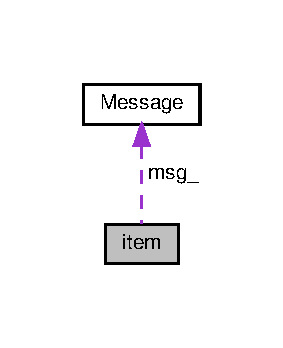
\includegraphics[width=136pt]{structitem__coll__graph}
\end{center}
\end{figure}


The documentation for this struct was generated from the following file\+:\begin{DoxyCompactItemize}
\item 
\hyperlink{Message_8hpp}{Message.\+hpp}\end{DoxyCompactItemize}

\hypertarget{structliveData}{}\section{live\+Data Struct Reference}
\label{structliveData}\index{live\+Data@{live\+Data}}


Inheritance diagram for live\+Data\+:\nopagebreak
\begin{figure}[H]
\begin{center}
\leavevmode
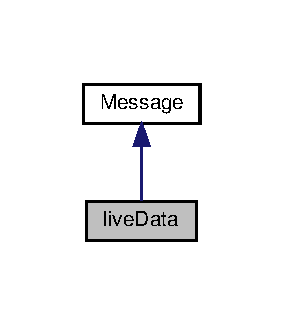
\includegraphics[width=136pt]{structliveData__inherit__graph}
\end{center}
\end{figure}


Collaboration diagram for live\+Data\+:\nopagebreak
\begin{figure}[H]
\begin{center}
\leavevmode
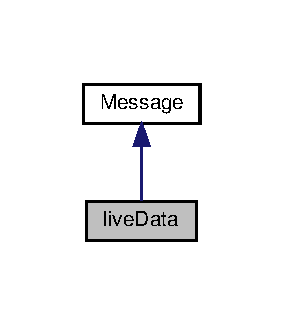
\includegraphics[width=136pt]{structliveData__coll__graph}
\end{center}
\end{figure}


The documentation for this struct was generated from the following file\+:\begin{DoxyCompactItemize}
\item 
thread\+Functionality.\+hpp\end{DoxyCompactItemize}

\hypertarget{classlockUnit}{}\section{lock\+Unit Class Reference}
\label{classlockUnit}\index{lock\+Unit@{lock\+Unit}}


The documentation for this class was generated from the following files\+:\begin{DoxyCompactItemize}
\item 
Lock\+Unit.\+hpp\item 
Lock\+Unit.\+cpp\end{DoxyCompactItemize}

\hypertarget{classMessage}{}\section{Message Class Reference}
\label{classMessage}\index{Message@{Message}}


Inheritance diagram for Message\+:\nopagebreak
\begin{figure}[H]
\begin{center}
\leavevmode
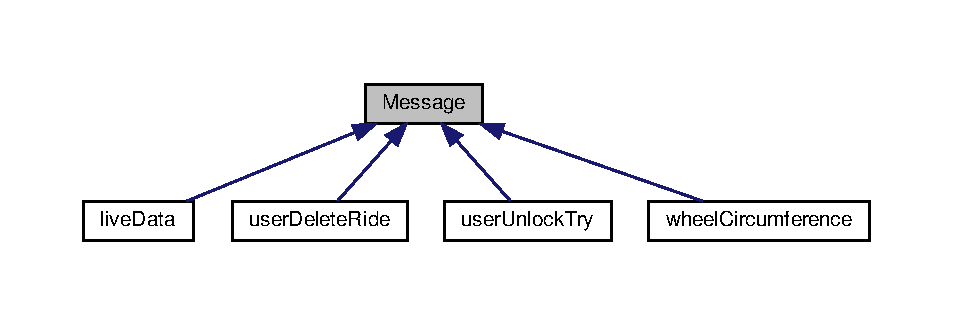
\includegraphics[width=350pt]{classMessage__inherit__graph}
\end{center}
\end{figure}


The documentation for this class was generated from the following file\+:\begin{DoxyCompactItemize}
\item 
\hyperlink{Message_8hpp}{Message.\+hpp}\end{DoxyCompactItemize}

\hypertarget{classMessageQ}{}\section{MessageQ Class Reference}
\label{classMessageQ}\index{MessageQ@{MessageQ}}
\subsection*{Public Member Functions}
\begin{DoxyCompactItemize}
\item 
\hyperlink{classMessageQ_aab147ebcd0b13fb87c5767738636ae1b}{MessageQ} (unsigned long max\+Q\+Capacity=20)
\begin{DoxyCompactList}\small\item\em Klassens constructor Initialiserer køens størrelse. \end{DoxyCompactList}\item 
void \hyperlink{classMessageQ_a7914a62e73bbdefa25db31e7279dd7bb}{send} (unsigned long ID, \hyperlink{classMessage}{Message} $\ast$msg=nullptr)
\begin{DoxyCompactList}\small\item\em Lægger besked ind i køen. \end{DoxyCompactList}\item 
\hyperlink{classMessage}{Message} $\ast$ \hyperlink{classMessageQ_a188ce4eab91cfe6dc0362d97f2a82f6e}{receive} (unsigned long \&ID)
\begin{DoxyCompactList}\small\item\em Henter en besked fra køen. \end{DoxyCompactList}\end{DoxyCompactItemize}


\subsection{Constructor \& Destructor Documentation}
\mbox{\Hypertarget{classMessageQ_aab147ebcd0b13fb87c5767738636ae1b}\label{classMessageQ_aab147ebcd0b13fb87c5767738636ae1b}} 
\index{MessageQ@{MessageQ}!MessageQ@{MessageQ}}
\index{MessageQ@{MessageQ}!MessageQ@{MessageQ}}
\subsubsection{\texorpdfstring{Message\+Q()}{MessageQ()}}
{\footnotesize\ttfamily Message\+Q\+::\+MessageQ (\begin{DoxyParamCaption}\item[{unsigned long}]{max\+Q\+Capacity = {\ttfamily 20} }\end{DoxyParamCaption})\hspace{0.3cm}{\ttfamily [inline]}}



Klassens constructor Initialiserer køens størrelse. 


\begin{DoxyParams}{Parameters}
{\em Max\+Q\+Capacity} & Køens størrelse \\
\hline
\end{DoxyParams}


\subsection{Member Function Documentation}
\mbox{\Hypertarget{classMessageQ_a188ce4eab91cfe6dc0362d97f2a82f6e}\label{classMessageQ_a188ce4eab91cfe6dc0362d97f2a82f6e}} 
\index{MessageQ@{MessageQ}!receive@{receive}}
\index{receive@{receive}!MessageQ@{MessageQ}}
\subsubsection{\texorpdfstring{receive()}{receive()}}
{\footnotesize\ttfamily \hyperlink{classMessage}{Message}$\ast$ Message\+Q\+::receive (\begin{DoxyParamCaption}\item[{unsigned long \&}]{ID }\end{DoxyParamCaption})\hspace{0.3cm}{\ttfamily [inline]}}



Henter en besked fra køen. 


\begin{DoxyParams}{Parameters}
{\em ID} & Reference til ID\textquotesingle{}et på den besked, der hentes fra køen \\
\hline
\end{DoxyParams}
\begin{DoxyReturn}{Returns}
Returnerer en pointer til dataene for den besked, der hentes fra køen. 
\end{DoxyReturn}
\mbox{\Hypertarget{classMessageQ_a7914a62e73bbdefa25db31e7279dd7bb}\label{classMessageQ_a7914a62e73bbdefa25db31e7279dd7bb}} 
\index{MessageQ@{MessageQ}!send@{send}}
\index{send@{send}!MessageQ@{MessageQ}}
\subsubsection{\texorpdfstring{send()}{send()}}
{\footnotesize\ttfamily void Message\+Q\+::send (\begin{DoxyParamCaption}\item[{unsigned long}]{ID,  }\item[{\hyperlink{classMessage}{Message} $\ast$}]{msg = {\ttfamily nullptr} }\end{DoxyParamCaption})\hspace{0.3cm}{\ttfamily [inline]}}



Lægger besked ind i køen. 


\begin{DoxyParams}{Parameters}
{\em ID} & ID\textquotesingle{}et på det event, der lægges ind i køen \\
\hline
{\em msg} & Dataene for det event, der lægges ind i køen. Sættes til nullptr, hvis ikke der sendes noget data. \\
\hline
\end{DoxyParams}
\begin{DoxyReturn}{Returns}

\end{DoxyReturn}


The documentation for this class was generated from the following file\+:\begin{DoxyCompactItemize}
\item 
\hyperlink{MessageQ_8hpp}{Message\+Q.\+hpp}\end{DoxyCompactItemize}

\hypertarget{classRideData}{}\section{Ride\+Data Class Reference}
\label{classRideData}\index{Ride\+Data@{Ride\+Data}}
\subsection*{Public Member Functions}
\begin{DoxyCompactItemize}
\item 
\mbox{\Hypertarget{classRideData_a74b3ac8999a7d0cb153e16fee0831161}\label{classRideData_a74b3ac8999a7d0cb153e16fee0831161}} 
\hyperlink{classRideData_a74b3ac8999a7d0cb153e16fee0831161}{Ride\+Data} ()
\begin{DoxyCompactList}\small\item\em Klassens constructor. Nulstiller alle variabler. \end{DoxyCompactList}\item 
\mbox{\Hypertarget{classRideData_a9c7f9d737269d475ec544079993a021e}\label{classRideData_a9c7f9d737269d475ec544079993a021e}} 
void \hyperlink{classRideData_a9c7f9d737269d475ec544079993a021e}{set\+Start\+Time} ()
\begin{DoxyCompactList}\small\item\em Sætter start tidspunkt på turen Benytter biblioteket time.\+h til at sætte turens starttidspunkt til det nuværende tidspunkt på R\+PI\textquotesingle{}en. \end{DoxyCompactList}\item 
\mbox{\Hypertarget{classRideData_af99bbf3658597b735fb9635ee00bb699}\label{classRideData_af99bbf3658597b735fb9635ee00bb699}} 
void \hyperlink{classRideData_af99bbf3658597b735fb9635ee00bb699}{set\+Endtime} ()
\begin{DoxyCompactList}\small\item\em Sætter sluttidspunkt på turen Benytter biblioteket time.\+h til at sætte turens sluttidspunkt til det nuværnde tidspunkt på R\+PI\textquotesingle{}en. \end{DoxyCompactList}\item 
\mbox{\Hypertarget{classRideData_a8664eef8bdd2942e8b18d24fbfe202f1}\label{classRideData_a8664eef8bdd2942e8b18d24fbfe202f1}} 
void \hyperlink{classRideData_a8664eef8bdd2942e8b18d24fbfe202f1}{set\+Date} ()
\begin{DoxyCompactList}\small\item\em Sætter datoen på turen Benytter biblioteket time.\+h til at sætte turens dato til den nuværnde dato på R\+PI\textquotesingle{}en. \end{DoxyCompactList}\item 
void \hyperlink{classRideData_a0290811130a17ab192e4c89068a48df9}{set\+ID} (int)
\begin{DoxyCompactList}\small\item\em Giver turen et ID Tager en int id som den så bruger som ID\textquotesingle{}et på turen. \end{DoxyCompactList}\item 
\mbox{\Hypertarget{classRideData_aaa4e995f1a17e0a92e7db6dc3cd7bbdb}\label{classRideData_aaa4e995f1a17e0a92e7db6dc3cd7bbdb}} 
void \hyperlink{classRideData_aaa4e995f1a17e0a92e7db6dc3cd7bbdb}{reset\+Values} ()
\begin{DoxyCompactList}\small\item\em Nulstiller de top\+Speed og avrage\+Speed Bruges når der starter en ny tur. \end{DoxyCompactList}\item 
void \hyperlink{classRideData_a0b805e6b56d07d574902ca37eed99758}{update\+Values} (int current\+Speed, int distance)
\begin{DoxyCompactList}\small\item\em Sætter distance, top\+Speed og avrage\+Speed For besked om hvor langt der er kørt og hvilken hastighed der er lige nu. Så sætter den distance til den distance den får. Hvis den nye hastighed er større end den gamle top\+Speed sætter den en ny top speed. Det sidste den gør er at udregne en gennemsnitsfart og så gemme den. \end{DoxyCompactList}\item 
\mbox{\Hypertarget{classRideData_a920d73fd13d8d0f19a66b03221669e13}\label{classRideData_a920d73fd13d8d0f19a66b03221669e13}} 
float \hyperlink{classRideData_a920d73fd13d8d0f19a66b03221669e13}{get\+Average\+Speed} ()
\begin{DoxyCompactList}\small\item\em Returnere avrage\+Speed. \end{DoxyCompactList}\item 
\mbox{\Hypertarget{classRideData_a695105f79682d98c02d38755744f9750}\label{classRideData_a695105f79682d98c02d38755744f9750}} 
int \hyperlink{classRideData_a695105f79682d98c02d38755744f9750}{get\+Top\+Speed} ()
\begin{DoxyCompactList}\small\item\em Returnere Top\+Speed. \end{DoxyCompactList}\item 
\mbox{\Hypertarget{classRideData_af72f4687f32b94d4f2d6e8cd59023b24}\label{classRideData_af72f4687f32b94d4f2d6e8cd59023b24}} 
int \hyperlink{classRideData_af72f4687f32b94d4f2d6e8cd59023b24}{get\+Distance} ()
\begin{DoxyCompactList}\small\item\em Returnere Distance. \end{DoxyCompactList}\item 
\mbox{\Hypertarget{classRideData_abb4c61080f8bb39388508b36605f4723}\label{classRideData_abb4c61080f8bb39388508b36605f4723}} 
string \hyperlink{classRideData_abb4c61080f8bb39388508b36605f4723}{get\+Start\+Time} ()
\begin{DoxyCompactList}\small\item\em Returnere Start\+Time. \end{DoxyCompactList}\item 
\mbox{\Hypertarget{classRideData_ab923d5c15bfe60ee62669b79bddbf1f5}\label{classRideData_ab923d5c15bfe60ee62669b79bddbf1f5}} 
string \hyperlink{classRideData_ab923d5c15bfe60ee62669b79bddbf1f5}{get\+End\+Time} ()
\begin{DoxyCompactList}\small\item\em Returnere End\+Time. \end{DoxyCompactList}\item 
\mbox{\Hypertarget{classRideData_a5bdfbd14490a8978865e0018c12d40d7}\label{classRideData_a5bdfbd14490a8978865e0018c12d40d7}} 
string \hyperlink{classRideData_a5bdfbd14490a8978865e0018c12d40d7}{get\+Date} ()
\begin{DoxyCompactList}\small\item\em Returnere Data. \end{DoxyCompactList}\item 
\mbox{\Hypertarget{classRideData_a75d2becd25de9eaef2e4fcbafc66b66f}\label{classRideData_a75d2becd25de9eaef2e4fcbafc66b66f}} 
int \hyperlink{classRideData_a75d2becd25de9eaef2e4fcbafc66b66f}{get\+ID} ()
\begin{DoxyCompactList}\small\item\em Returnere ID. \end{DoxyCompactList}\end{DoxyCompactItemize}


\subsection{Member Function Documentation}
\mbox{\Hypertarget{classRideData_a0290811130a17ab192e4c89068a48df9}\label{classRideData_a0290811130a17ab192e4c89068a48df9}} 
\index{Ride\+Data@{Ride\+Data}!set\+ID@{set\+ID}}
\index{set\+ID@{set\+ID}!Ride\+Data@{Ride\+Data}}
\subsubsection{\texorpdfstring{set\+I\+D()}{setID()}}
{\footnotesize\ttfamily void Ride\+Data\+::set\+ID (\begin{DoxyParamCaption}\item[{int}]{id }\end{DoxyParamCaption})}



Giver turen et ID Tager en int id som den så bruger som ID\textquotesingle{}et på turen. 


\begin{DoxyParams}{Parameters}
{\em int} & id, ID på turen \\
\hline
\end{DoxyParams}
\mbox{\Hypertarget{classRideData_a0b805e6b56d07d574902ca37eed99758}\label{classRideData_a0b805e6b56d07d574902ca37eed99758}} 
\index{Ride\+Data@{Ride\+Data}!update\+Values@{update\+Values}}
\index{update\+Values@{update\+Values}!Ride\+Data@{Ride\+Data}}
\subsubsection{\texorpdfstring{update\+Values()}{updateValues()}}
{\footnotesize\ttfamily void Ride\+Data\+::update\+Values (\begin{DoxyParamCaption}\item[{int}]{current\+Speed,  }\item[{int}]{distance }\end{DoxyParamCaption})}



Sætter distance, top\+Speed og avrage\+Speed For besked om hvor langt der er kørt og hvilken hastighed der er lige nu. Så sætter den distance til den distance den får. Hvis den nye hastighed er større end den gamle top\+Speed sætter den en ny top speed. Det sidste den gør er at udregne en gennemsnitsfart og så gemme den. 


\begin{DoxyParams}{Parameters}
{\em int} & current\+Speed, hastigheden lige nu \\
\hline
{\em int} & distance, hvor langt der er kørt \\
\hline
\end{DoxyParams}


The documentation for this class was generated from the following files\+:\begin{DoxyCompactItemize}
\item 
\hyperlink{RideData_8hpp}{Ride\+Data.\+hpp}\item 
\hyperlink{RideData_8cpp}{Ride\+Data.\+cpp}\end{DoxyCompactItemize}

\hypertarget{classsensorUnit}{}\section{sensor\+Unit Class Reference}
\label{classsensorUnit}\index{sensor\+Unit@{sensor\+Unit}}
\subsection*{Public Member Functions}
\begin{DoxyCompactItemize}
\item 
\hyperlink{classsensorUnit_a820a3a2b5353cbb927c109d45c194541}{sensor\+Unit} (\hyperlink{classserialUnit}{serial\+Unit} $\ast$\hyperlink{classserialUnit}{serial\+Unit})
\begin{DoxyCompactList}\small\item\em kort beskrivelse lang beskrivelse, lang beskrivelse, lang beskrivelse, lang beskrivelse, lang beskrivelse, lang beskrivelse \end{DoxyCompactList}\item 
\hyperlink{classsensorUnit_a1e606f860650fc1d62af09b7423a299d}{$\sim$sensor\+Unit} ()
\begin{DoxyCompactList}\small\item\em kort beskrivelse lang beskrivelse, lang beskrivelse, lang beskrivelse, lang beskrivelse, lang beskrivelse, lang beskrivelse \end{DoxyCompactList}\item 
void \hyperlink{classsensorUnit_ad5a61b8eb08a866d7a94c7bb4149a172}{pull} (uint8\+\_\+t $\ast$retrieve\+Buffer)
\begin{DoxyCompactList}\small\item\em kort beskrivelse lang beskrivelse, lang beskrivelse, lang beskrivelse, lang beskrivelse, lang beskrivelse, lang beskrivelse \end{DoxyCompactList}\item 
void \hyperlink{classsensorUnit_af089bd3cff5b63b7bc287cff2a7fb90f}{slave\+Puller\+To\+Dispatcher} (uint8\+\_\+t $\ast$buffer\+Received)
\begin{DoxyCompactList}\small\item\em kort beskrivelse lang beskrivelse, lang beskrivelse, lang beskrivelse, lang beskrivelse, lang beskrivelse, lang beskrivelse \end{DoxyCompactList}\item 
void \hyperlink{classsensorUnit_af597dff1d9bc84a5ab9b1b76ca38f00e}{slave\+Puller\+Thread\+Func} ()
\begin{DoxyCompactList}\small\item\em kort beskrivelse lang beskrivelse, lang beskrivelse, lang beskrivelse, lang beskrivelse, lang beskrivelse, lang beskrivelse \end{DoxyCompactList}\item 
int \hyperlink{classsensorUnit_aeb3f83f3e41d1a23974cf9d8537cf3f6}{set\+Wheel\+Circ} (int wheel\+Circ\+In\+Centi\+Meters)
\begin{DoxyCompactList}\small\item\em kort beskrivelse lang beskrivelse, lang beskrivelse, lang beskrivelse, lang beskrivelse, lang beskrivelse, lang beskrivelse \end{DoxyCompactList}\end{DoxyCompactItemize}


\subsection{Constructor \& Destructor Documentation}
\mbox{\Hypertarget{classsensorUnit_a820a3a2b5353cbb927c109d45c194541}\label{classsensorUnit_a820a3a2b5353cbb927c109d45c194541}} 
\index{sensor\+Unit@{sensor\+Unit}!sensor\+Unit@{sensor\+Unit}}
\index{sensor\+Unit@{sensor\+Unit}!sensor\+Unit@{sensor\+Unit}}
\subsubsection{\texorpdfstring{sensor\+Unit()}{sensorUnit()}}
{\footnotesize\ttfamily sensor\+Unit\+::sensor\+Unit (\begin{DoxyParamCaption}\item[{\hyperlink{classserialUnit}{serial\+Unit} $\ast$}]{serial\+Unit }\end{DoxyParamCaption})}



kort beskrivelse lang beskrivelse, lang beskrivelse, lang beskrivelse, lang beskrivelse, lang beskrivelse, lang beskrivelse 


\begin{DoxyParams}{Parameters}
{\em param1} & beskrivelse af param1 \\
\hline
{\em param2} & beskrivelse af param2 \\
\hline
\end{DoxyParams}
\begin{DoxyReturn}{Returns}
beskrivelse af metodens returværdi 
\end{DoxyReturn}
\mbox{\Hypertarget{classsensorUnit_a1e606f860650fc1d62af09b7423a299d}\label{classsensorUnit_a1e606f860650fc1d62af09b7423a299d}} 
\index{sensor\+Unit@{sensor\+Unit}!````~sensor\+Unit@{$\sim$sensor\+Unit}}
\index{````~sensor\+Unit@{$\sim$sensor\+Unit}!sensor\+Unit@{sensor\+Unit}}
\subsubsection{\texorpdfstring{$\sim$sensor\+Unit()}{~sensorUnit()}}
{\footnotesize\ttfamily sensor\+Unit\+::$\sim$sensor\+Unit (\begin{DoxyParamCaption}{ }\end{DoxyParamCaption})}



kort beskrivelse lang beskrivelse, lang beskrivelse, lang beskrivelse, lang beskrivelse, lang beskrivelse, lang beskrivelse 


\begin{DoxyParams}{Parameters}
{\em param1} & beskrivelse af param1 \\
\hline
{\em param2} & beskrivelse af param2 \\
\hline
\end{DoxyParams}
\begin{DoxyReturn}{Returns}
beskrivelse af metodens returværdi 
\end{DoxyReturn}


\subsection{Member Function Documentation}
\mbox{\Hypertarget{classsensorUnit_ad5a61b8eb08a866d7a94c7bb4149a172}\label{classsensorUnit_ad5a61b8eb08a866d7a94c7bb4149a172}} 
\index{sensor\+Unit@{sensor\+Unit}!pull@{pull}}
\index{pull@{pull}!sensor\+Unit@{sensor\+Unit}}
\subsubsection{\texorpdfstring{pull()}{pull()}}
{\footnotesize\ttfamily void sensor\+Unit\+::pull (\begin{DoxyParamCaption}\item[{uint8\+\_\+t $\ast$}]{retrieve\+Buffer }\end{DoxyParamCaption})}



kort beskrivelse lang beskrivelse, lang beskrivelse, lang beskrivelse, lang beskrivelse, lang beskrivelse, lang beskrivelse 


\begin{DoxyParams}{Parameters}
{\em param1} & beskrivelse af param1 \\
\hline
{\em param2} & beskrivelse af param2 \\
\hline
\end{DoxyParams}
\begin{DoxyReturn}{Returns}
beskrivelse af metodens returværdi 
\end{DoxyReturn}
\mbox{\Hypertarget{classsensorUnit_aeb3f83f3e41d1a23974cf9d8537cf3f6}\label{classsensorUnit_aeb3f83f3e41d1a23974cf9d8537cf3f6}} 
\index{sensor\+Unit@{sensor\+Unit}!set\+Wheel\+Circ@{set\+Wheel\+Circ}}
\index{set\+Wheel\+Circ@{set\+Wheel\+Circ}!sensor\+Unit@{sensor\+Unit}}
\subsubsection{\texorpdfstring{set\+Wheel\+Circ()}{setWheelCirc()}}
{\footnotesize\ttfamily int sensor\+Unit\+::set\+Wheel\+Circ (\begin{DoxyParamCaption}\item[{int}]{wheel\+Circ\+In\+Centi\+Meters }\end{DoxyParamCaption})}



kort beskrivelse lang beskrivelse, lang beskrivelse, lang beskrivelse, lang beskrivelse, lang beskrivelse, lang beskrivelse 


\begin{DoxyParams}{Parameters}
{\em param1} & beskrivelse af param1 \\
\hline
{\em param2} & beskrivelse af param2 \\
\hline
\end{DoxyParams}
\begin{DoxyReturn}{Returns}
beskrivelse af metodens returværdi 
\end{DoxyReturn}
\mbox{\Hypertarget{classsensorUnit_af597dff1d9bc84a5ab9b1b76ca38f00e}\label{classsensorUnit_af597dff1d9bc84a5ab9b1b76ca38f00e}} 
\index{sensor\+Unit@{sensor\+Unit}!slave\+Puller\+Thread\+Func@{slave\+Puller\+Thread\+Func}}
\index{slave\+Puller\+Thread\+Func@{slave\+Puller\+Thread\+Func}!sensor\+Unit@{sensor\+Unit}}
\subsubsection{\texorpdfstring{slave\+Puller\+Thread\+Func()}{slavePullerThreadFunc()}}
{\footnotesize\ttfamily void sensor\+Unit\+::slave\+Puller\+Thread\+Func (\begin{DoxyParamCaption}{ }\end{DoxyParamCaption})}



kort beskrivelse lang beskrivelse, lang beskrivelse, lang beskrivelse, lang beskrivelse, lang beskrivelse, lang beskrivelse 


\begin{DoxyParams}{Parameters}
{\em param1} & beskrivelse af param1 \\
\hline
{\em param2} & beskrivelse af param2 \\
\hline
\end{DoxyParams}
\begin{DoxyReturn}{Returns}
beskrivelse af metodens returværdi 
\end{DoxyReturn}
\mbox{\Hypertarget{classsensorUnit_af089bd3cff5b63b7bc287cff2a7fb90f}\label{classsensorUnit_af089bd3cff5b63b7bc287cff2a7fb90f}} 
\index{sensor\+Unit@{sensor\+Unit}!slave\+Puller\+To\+Dispatcher@{slave\+Puller\+To\+Dispatcher}}
\index{slave\+Puller\+To\+Dispatcher@{slave\+Puller\+To\+Dispatcher}!sensor\+Unit@{sensor\+Unit}}
\subsubsection{\texorpdfstring{slave\+Puller\+To\+Dispatcher()}{slavePullerToDispatcher()}}
{\footnotesize\ttfamily void sensor\+Unit\+::slave\+Puller\+To\+Dispatcher (\begin{DoxyParamCaption}\item[{uint8\+\_\+t $\ast$}]{buffer\+Received }\end{DoxyParamCaption})}



kort beskrivelse lang beskrivelse, lang beskrivelse, lang beskrivelse, lang beskrivelse, lang beskrivelse, lang beskrivelse 


\begin{DoxyParams}{Parameters}
{\em param1} & beskrivelse af param1 \\
\hline
{\em param2} & beskrivelse af param2 \\
\hline
\end{DoxyParams}
\begin{DoxyReturn}{Returns}
beskrivelse af metodens returværdi 
\end{DoxyReturn}


The documentation for this class was generated from the following files\+:\begin{DoxyCompactItemize}
\item 
Sensor\+Unit.\+hpp\item 
Sensor\+Unit.\+cpp\end{DoxyCompactItemize}

\hypertarget{classserialUnit}{}\section{serial\+Unit Class Reference}
\label{classserialUnit}\index{serial\+Unit@{serial\+Unit}}


Inheritance diagram for serial\+Unit\+:\nopagebreak
\begin{figure}[H]
\begin{center}
\leavevmode
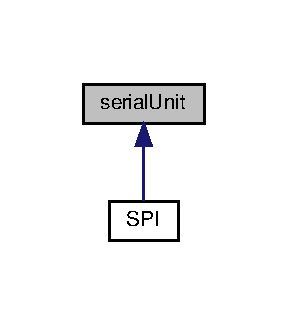
\includegraphics[width=138pt]{classserialUnit__inherit__graph}
\end{center}
\end{figure}
\subsection*{Public Member Functions}
\begin{DoxyCompactItemize}
\item 
\hyperlink{classserialUnit_af26f4292b42cd782520962aebc9d708e}{serial\+Unit} ()
\begin{DoxyCompactList}\small\item\em kort beskrivelse lang beskrivelse, lang beskrivelse, lang beskrivelse, lang beskrivelse, lang beskrivelse, lang beskrivelse \end{DoxyCompactList}\item 
virtual \hyperlink{classserialUnit_a1e6211e2fe4b241d3f2e2dc116435b7d}{$\sim$serial\+Unit} ()=0
\begin{DoxyCompactList}\small\item\em kort beskrivelse lang beskrivelse, lang beskrivelse, lang beskrivelse, lang beskrivelse, lang beskrivelse, lang beskrivelse \end{DoxyCompactList}\item 
virtual int \hyperlink{classserialUnit_a5d5573f6d367d8e191df6b8044a81a62}{read\+And\+Write} (int message\+Len, int optional\+Arg)=0
\begin{DoxyCompactList}\small\item\em kort beskrivelse lang beskrivelse, lang beskrivelse, lang beskrivelse, lang beskrivelse, lang beskrivelse, lang beskrivelse \end{DoxyCompactList}\item 
virtual void \hyperlink{classserialUnit_a88db4b94632c6ab70933bb32f105821d}{get\+Value\+Of\+Rx\+Buffer} (uint8\+\_\+t $\ast$call\+Back\+Buffer)=0
\begin{DoxyCompactList}\small\item\em kort beskrivelse lang beskrivelse, lang beskrivelse, lang beskrivelse, lang beskrivelse, lang beskrivelse, lang beskrivelse \end{DoxyCompactList}\item 
virtual void \hyperlink{classserialUnit_a759db776a18c097ce85652d41d46b943}{set\+Value\+Of\+Tx\+Buffer} (std\+::string tx)=0
\begin{DoxyCompactList}\small\item\em kort beskrivelse lang beskrivelse, lang beskrivelse, lang beskrivelse, lang beskrivelse, lang beskrivelse, lang beskrivelse \end{DoxyCompactList}\item 
virtual void \hyperlink{classserialUnit_a1e70c25a8057dd67330022a292144900}{set\+Value\+Of\+Tx\+Buffer} (uint8\+\_\+t for\+Index0, uint8\+\_\+t for\+Index1, uint8\+\_\+t for\+Index2, uint8\+\_\+t for\+Index3)=0
\begin{DoxyCompactList}\small\item\em kort beskrivelse lang beskrivelse, lang beskrivelse, lang beskrivelse, lang beskrivelse, lang beskrivelse, lang beskrivelse \end{DoxyCompactList}\item 
virtual void \hyperlink{classserialUnit_a3d529e2d2c5908ecf8106ff796e4c3eb}{print\+Rx\+To\+Screen} ()=0
\begin{DoxyCompactList}\small\item\em kort beskrivelse lang beskrivelse, lang beskrivelse, lang beskrivelse, lang beskrivelse, lang beskrivelse, lang beskrivelse \end{DoxyCompactList}\item 
virtual void \hyperlink{classserialUnit_a48e5dcf17a5a551351d7569c43cf96ad}{print\+Tx\+To\+Screen} ()=0
\begin{DoxyCompactList}\small\item\em kort beskrivelse lang beskrivelse, lang beskrivelse, lang beskrivelse, lang beskrivelse, lang beskrivelse, lang beskrivelse \end{DoxyCompactList}\end{DoxyCompactItemize}


\subsection{Constructor \& Destructor Documentation}
\mbox{\Hypertarget{classserialUnit_af26f4292b42cd782520962aebc9d708e}\label{classserialUnit_af26f4292b42cd782520962aebc9d708e}} 
\index{serial\+Unit@{serial\+Unit}!serial\+Unit@{serial\+Unit}}
\index{serial\+Unit@{serial\+Unit}!serial\+Unit@{serial\+Unit}}
\subsubsection{\texorpdfstring{serial\+Unit()}{serialUnit()}}
{\footnotesize\ttfamily serial\+Unit\+::serial\+Unit (\begin{DoxyParamCaption}{ }\end{DoxyParamCaption})}



kort beskrivelse lang beskrivelse, lang beskrivelse, lang beskrivelse, lang beskrivelse, lang beskrivelse, lang beskrivelse 


\begin{DoxyParams}{Parameters}
{\em param1} & beskrivelse af param1 \\
\hline
{\em param2} & beskrivelse af param2 \\
\hline
\end{DoxyParams}
\begin{DoxyReturn}{Returns}
beskrivelse af metodens returværdi 
\end{DoxyReturn}
\mbox{\Hypertarget{classserialUnit_a1e6211e2fe4b241d3f2e2dc116435b7d}\label{classserialUnit_a1e6211e2fe4b241d3f2e2dc116435b7d}} 
\index{serial\+Unit@{serial\+Unit}!````~serial\+Unit@{$\sim$serial\+Unit}}
\index{````~serial\+Unit@{$\sim$serial\+Unit}!serial\+Unit@{serial\+Unit}}
\subsubsection{\texorpdfstring{$\sim$serial\+Unit()}{~serialUnit()}}
{\footnotesize\ttfamily serial\+Unit\+::$\sim$serial\+Unit (\begin{DoxyParamCaption}{ }\end{DoxyParamCaption})\hspace{0.3cm}{\ttfamily [pure virtual]}}



kort beskrivelse lang beskrivelse, lang beskrivelse, lang beskrivelse, lang beskrivelse, lang beskrivelse, lang beskrivelse 


\begin{DoxyParams}{Parameters}
{\em param1} & beskrivelse af param1 \\
\hline
{\em param2} & beskrivelse af param2 \\
\hline
\end{DoxyParams}
\begin{DoxyReturn}{Returns}
beskrivelse af metodens returværdi 
\end{DoxyReturn}


\subsection{Member Function Documentation}
\mbox{\Hypertarget{classserialUnit_a88db4b94632c6ab70933bb32f105821d}\label{classserialUnit_a88db4b94632c6ab70933bb32f105821d}} 
\index{serial\+Unit@{serial\+Unit}!get\+Value\+Of\+Rx\+Buffer@{get\+Value\+Of\+Rx\+Buffer}}
\index{get\+Value\+Of\+Rx\+Buffer@{get\+Value\+Of\+Rx\+Buffer}!serial\+Unit@{serial\+Unit}}
\subsubsection{\texorpdfstring{get\+Value\+Of\+Rx\+Buffer()}{getValueOfRxBuffer()}}
{\footnotesize\ttfamily virtual void serial\+Unit\+::get\+Value\+Of\+Rx\+Buffer (\begin{DoxyParamCaption}\item[{uint8\+\_\+t $\ast$}]{call\+Back\+Buffer }\end{DoxyParamCaption})\hspace{0.3cm}{\ttfamily [pure virtual]}}



kort beskrivelse lang beskrivelse, lang beskrivelse, lang beskrivelse, lang beskrivelse, lang beskrivelse, lang beskrivelse 


\begin{DoxyParams}{Parameters}
{\em param1} & beskrivelse af param1 \\
\hline
{\em param2} & beskrivelse af param2 \\
\hline
\end{DoxyParams}
\begin{DoxyReturn}{Returns}
beskrivelse af metodens returværdi 
\end{DoxyReturn}


Implemented in \hyperlink{classSPI_ad468d421e9c82453957c5ee7ea7d5b9d}{S\+PI}.

\mbox{\Hypertarget{classserialUnit_a3d529e2d2c5908ecf8106ff796e4c3eb}\label{classserialUnit_a3d529e2d2c5908ecf8106ff796e4c3eb}} 
\index{serial\+Unit@{serial\+Unit}!print\+Rx\+To\+Screen@{print\+Rx\+To\+Screen}}
\index{print\+Rx\+To\+Screen@{print\+Rx\+To\+Screen}!serial\+Unit@{serial\+Unit}}
\subsubsection{\texorpdfstring{print\+Rx\+To\+Screen()}{printRxToScreen()}}
{\footnotesize\ttfamily virtual void serial\+Unit\+::print\+Rx\+To\+Screen (\begin{DoxyParamCaption}{ }\end{DoxyParamCaption})\hspace{0.3cm}{\ttfamily [pure virtual]}}



kort beskrivelse lang beskrivelse, lang beskrivelse, lang beskrivelse, lang beskrivelse, lang beskrivelse, lang beskrivelse 


\begin{DoxyParams}{Parameters}
{\em param1} & beskrivelse af param1 \\
\hline
{\em param2} & beskrivelse af param2 \\
\hline
\end{DoxyParams}
\begin{DoxyReturn}{Returns}
beskrivelse af metodens returværdi 
\end{DoxyReturn}


Implemented in \hyperlink{classSPI_a33d7fcfab7e5962dd1392aecfd58eaca}{S\+PI}.

\mbox{\Hypertarget{classserialUnit_a48e5dcf17a5a551351d7569c43cf96ad}\label{classserialUnit_a48e5dcf17a5a551351d7569c43cf96ad}} 
\index{serial\+Unit@{serial\+Unit}!print\+Tx\+To\+Screen@{print\+Tx\+To\+Screen}}
\index{print\+Tx\+To\+Screen@{print\+Tx\+To\+Screen}!serial\+Unit@{serial\+Unit}}
\subsubsection{\texorpdfstring{print\+Tx\+To\+Screen()}{printTxToScreen()}}
{\footnotesize\ttfamily virtual void serial\+Unit\+::print\+Tx\+To\+Screen (\begin{DoxyParamCaption}{ }\end{DoxyParamCaption})\hspace{0.3cm}{\ttfamily [pure virtual]}}



kort beskrivelse lang beskrivelse, lang beskrivelse, lang beskrivelse, lang beskrivelse, lang beskrivelse, lang beskrivelse 


\begin{DoxyParams}{Parameters}
{\em param1} & beskrivelse af param1 \\
\hline
{\em param2} & beskrivelse af param2 \\
\hline
\end{DoxyParams}
\begin{DoxyReturn}{Returns}
beskrivelse af metodens returværdi 
\end{DoxyReturn}


Implemented in \hyperlink{classSPI_a54c4ecb02366f1e31d2e6f4aa6db8f7d}{S\+PI}.

\mbox{\Hypertarget{classserialUnit_a5d5573f6d367d8e191df6b8044a81a62}\label{classserialUnit_a5d5573f6d367d8e191df6b8044a81a62}} 
\index{serial\+Unit@{serial\+Unit}!read\+And\+Write@{read\+And\+Write}}
\index{read\+And\+Write@{read\+And\+Write}!serial\+Unit@{serial\+Unit}}
\subsubsection{\texorpdfstring{read\+And\+Write()}{readAndWrite()}}
{\footnotesize\ttfamily virtual int serial\+Unit\+::read\+And\+Write (\begin{DoxyParamCaption}\item[{int}]{message\+Len,  }\item[{int}]{optional\+Arg }\end{DoxyParamCaption})\hspace{0.3cm}{\ttfamily [pure virtual]}}



kort beskrivelse lang beskrivelse, lang beskrivelse, lang beskrivelse, lang beskrivelse, lang beskrivelse, lang beskrivelse 


\begin{DoxyParams}{Parameters}
{\em param1} & beskrivelse af param1 \\
\hline
{\em param2} & beskrivelse af param2 \\
\hline
\end{DoxyParams}
\begin{DoxyReturn}{Returns}
beskrivelse af metodens returværdi 
\end{DoxyReturn}


Implemented in \hyperlink{classSPI_ac50b3f5491e294aef6806f4e131cbd0e}{S\+PI}.

\mbox{\Hypertarget{classserialUnit_a759db776a18c097ce85652d41d46b943}\label{classserialUnit_a759db776a18c097ce85652d41d46b943}} 
\index{serial\+Unit@{serial\+Unit}!set\+Value\+Of\+Tx\+Buffer@{set\+Value\+Of\+Tx\+Buffer}}
\index{set\+Value\+Of\+Tx\+Buffer@{set\+Value\+Of\+Tx\+Buffer}!serial\+Unit@{serial\+Unit}}
\subsubsection{\texorpdfstring{set\+Value\+Of\+Tx\+Buffer()}{setValueOfTxBuffer()}\hspace{0.1cm}{\footnotesize\ttfamily [1/2]}}
{\footnotesize\ttfamily virtual void serial\+Unit\+::set\+Value\+Of\+Tx\+Buffer (\begin{DoxyParamCaption}\item[{std\+::string}]{tx }\end{DoxyParamCaption})\hspace{0.3cm}{\ttfamily [pure virtual]}}



kort beskrivelse lang beskrivelse, lang beskrivelse, lang beskrivelse, lang beskrivelse, lang beskrivelse, lang beskrivelse 


\begin{DoxyParams}{Parameters}
{\em param1} & beskrivelse af param1 \\
\hline
{\em param2} & beskrivelse af param2 \\
\hline
\end{DoxyParams}
\begin{DoxyReturn}{Returns}
beskrivelse af metodens returværdi 
\end{DoxyReturn}


Implemented in \hyperlink{classSPI_ad770b7e8e8ae678a2c3c5e2d2be6887a}{S\+PI}.

\mbox{\Hypertarget{classserialUnit_a1e70c25a8057dd67330022a292144900}\label{classserialUnit_a1e70c25a8057dd67330022a292144900}} 
\index{serial\+Unit@{serial\+Unit}!set\+Value\+Of\+Tx\+Buffer@{set\+Value\+Of\+Tx\+Buffer}}
\index{set\+Value\+Of\+Tx\+Buffer@{set\+Value\+Of\+Tx\+Buffer}!serial\+Unit@{serial\+Unit}}
\subsubsection{\texorpdfstring{set\+Value\+Of\+Tx\+Buffer()}{setValueOfTxBuffer()}\hspace{0.1cm}{\footnotesize\ttfamily [2/2]}}
{\footnotesize\ttfamily virtual void serial\+Unit\+::set\+Value\+Of\+Tx\+Buffer (\begin{DoxyParamCaption}\item[{uint8\+\_\+t}]{for\+Index0,  }\item[{uint8\+\_\+t}]{for\+Index1,  }\item[{uint8\+\_\+t}]{for\+Index2,  }\item[{uint8\+\_\+t}]{for\+Index3 }\end{DoxyParamCaption})\hspace{0.3cm}{\ttfamily [pure virtual]}}



kort beskrivelse lang beskrivelse, lang beskrivelse, lang beskrivelse, lang beskrivelse, lang beskrivelse, lang beskrivelse 


\begin{DoxyParams}{Parameters}
{\em param1} & beskrivelse af param1 \\
\hline
{\em param2} & beskrivelse af param2 \\
\hline
\end{DoxyParams}
\begin{DoxyReturn}{Returns}
beskrivelse af metodens returværdi 
\end{DoxyReturn}


Implemented in \hyperlink{classSPI_ad581e7b40a17f41f8d6db8dec97c9c4b}{S\+PI}.



The documentation for this class was generated from the following files\+:\begin{DoxyCompactItemize}
\item 
Serial\+Unit.\+hpp\item 
Serial\+Unit.\+cpp\end{DoxyCompactItemize}

\hypertarget{classSPI}{}\section{S\+PI Class Reference}
\label{classSPI}\index{S\+PI@{S\+PI}}


Inheritance diagram for S\+PI\+:\nopagebreak
\begin{figure}[H]
\begin{center}
\leavevmode
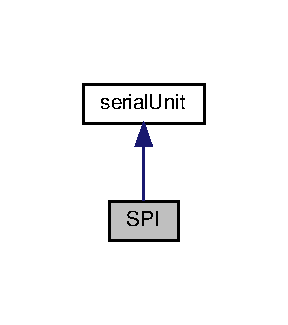
\includegraphics[width=138pt]{classSPI__inherit__graph}
\end{center}
\end{figure}


Collaboration diagram for S\+PI\+:\nopagebreak
\begin{figure}[H]
\begin{center}
\leavevmode
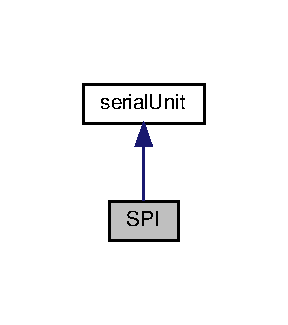
\includegraphics[width=138pt]{classSPI__coll__graph}
\end{center}
\end{figure}
\subsection*{Public Member Functions}
\begin{DoxyCompactItemize}
\item 
\hyperlink{classSPI_aa4928d013558671e0622e7320414ab77}{S\+PI} (int device\+Number, unsigned char bits\+Per\+Word, unsigned int speed)
\begin{DoxyCompactList}\small\item\em kort beskrivelse lang beskrivelse, lang beskrivelse, lang beskrivelse, lang beskrivelse, lang beskrivelse, lang beskrivelse \end{DoxyCompactList}\item 
virtual \hyperlink{classSPI_a6babebf1ea3e8ff0330f43a3e2312ac4}{$\sim$\+S\+PI} ()
\begin{DoxyCompactList}\small\item\em kort beskrivelse lang beskrivelse, lang beskrivelse, lang beskrivelse, lang beskrivelse, lang beskrivelse, lang beskrivelse \end{DoxyCompactList}\item 
virtual int \hyperlink{classSPI_ac50b3f5491e294aef6806f4e131cbd0e}{read\+And\+Write} (int message\+Len, int cs\+After\+Transfer)
\begin{DoxyCompactList}\small\item\em kort beskrivelse lang beskrivelse, lang beskrivelse, lang beskrivelse, lang beskrivelse, lang beskrivelse, lang beskrivelse \end{DoxyCompactList}\item 
virtual void \hyperlink{classSPI_ad468d421e9c82453957c5ee7ea7d5b9d}{get\+Value\+Of\+Rx\+Buffer} (uint8\+\_\+t $\ast$call\+Back\+Buffer)
\begin{DoxyCompactList}\small\item\em kort beskrivelse lang beskrivelse, lang beskrivelse, lang beskrivelse, lang beskrivelse, lang beskrivelse, lang beskrivelse \end{DoxyCompactList}\item 
virtual void \hyperlink{classSPI_ad770b7e8e8ae678a2c3c5e2d2be6887a}{set\+Value\+Of\+Tx\+Buffer} (std\+::string tx)
\begin{DoxyCompactList}\small\item\em kort beskrivelse lang beskrivelse, lang beskrivelse, lang beskrivelse, lang beskrivelse, lang beskrivelse, lang beskrivelse \end{DoxyCompactList}\item 
virtual void \hyperlink{classSPI_ad581e7b40a17f41f8d6db8dec97c9c4b}{set\+Value\+Of\+Tx\+Buffer} (uint8\+\_\+t for\+Index0, uint8\+\_\+t for\+Index1, uint8\+\_\+t for\+Index2, uint8\+\_\+t for\+Index3)
\begin{DoxyCompactList}\small\item\em kort beskrivelse lang beskrivelse, lang beskrivelse, lang beskrivelse, lang beskrivelse, lang beskrivelse, lang beskrivelse \end{DoxyCompactList}\item 
virtual void \hyperlink{classSPI_a33d7fcfab7e5962dd1392aecfd58eaca}{print\+Rx\+To\+Screen} ()
\begin{DoxyCompactList}\small\item\em kort beskrivelse lang beskrivelse, lang beskrivelse, lang beskrivelse, lang beskrivelse, lang beskrivelse, lang beskrivelse \end{DoxyCompactList}\item 
virtual void \hyperlink{classSPI_a54c4ecb02366f1e31d2e6f4aa6db8f7d}{print\+Tx\+To\+Screen} ()
\begin{DoxyCompactList}\small\item\em kort beskrivelse lang beskrivelse, lang beskrivelse, lang beskrivelse, lang beskrivelse, lang beskrivelse, lang beskrivelse \end{DoxyCompactList}\end{DoxyCompactItemize}


\subsection{Constructor \& Destructor Documentation}
\mbox{\Hypertarget{classSPI_aa4928d013558671e0622e7320414ab77}\label{classSPI_aa4928d013558671e0622e7320414ab77}} 
\index{S\+PI@{S\+PI}!S\+PI@{S\+PI}}
\index{S\+PI@{S\+PI}!S\+PI@{S\+PI}}
\subsubsection{\texorpdfstring{S\+P\+I()}{SPI()}}
{\footnotesize\ttfamily S\+P\+I\+::\+S\+PI (\begin{DoxyParamCaption}\item[{int}]{device\+Number,  }\item[{unsigned char}]{bits\+Per\+Word,  }\item[{unsigned int}]{speed }\end{DoxyParamCaption})}



kort beskrivelse lang beskrivelse, lang beskrivelse, lang beskrivelse, lang beskrivelse, lang beskrivelse, lang beskrivelse 


\begin{DoxyParams}{Parameters}
{\em param1} & beskrivelse af param1 \\
\hline
{\em param2} & beskrivelse af param2 \\
\hline
\end{DoxyParams}
\begin{DoxyReturn}{Returns}
beskrivelse af metodens returværdi 
\end{DoxyReturn}
\mbox{\Hypertarget{classSPI_a6babebf1ea3e8ff0330f43a3e2312ac4}\label{classSPI_a6babebf1ea3e8ff0330f43a3e2312ac4}} 
\index{S\+PI@{S\+PI}!````~S\+PI@{$\sim$\+S\+PI}}
\index{````~S\+PI@{$\sim$\+S\+PI}!S\+PI@{S\+PI}}
\subsubsection{\texorpdfstring{$\sim$\+S\+P\+I()}{~SPI()}}
{\footnotesize\ttfamily S\+P\+I\+::$\sim$\+S\+PI (\begin{DoxyParamCaption}{ }\end{DoxyParamCaption})\hspace{0.3cm}{\ttfamily [virtual]}}



kort beskrivelse lang beskrivelse, lang beskrivelse, lang beskrivelse, lang beskrivelse, lang beskrivelse, lang beskrivelse 


\begin{DoxyParams}{Parameters}
{\em param1} & beskrivelse af param1 \\
\hline
{\em param2} & beskrivelse af param2 \\
\hline
\end{DoxyParams}
\begin{DoxyReturn}{Returns}
beskrivelse af metodens returværdi 
\end{DoxyReturn}


\subsection{Member Function Documentation}
\mbox{\Hypertarget{classSPI_ad468d421e9c82453957c5ee7ea7d5b9d}\label{classSPI_ad468d421e9c82453957c5ee7ea7d5b9d}} 
\index{S\+PI@{S\+PI}!get\+Value\+Of\+Rx\+Buffer@{get\+Value\+Of\+Rx\+Buffer}}
\index{get\+Value\+Of\+Rx\+Buffer@{get\+Value\+Of\+Rx\+Buffer}!S\+PI@{S\+PI}}
\subsubsection{\texorpdfstring{get\+Value\+Of\+Rx\+Buffer()}{getValueOfRxBuffer()}}
{\footnotesize\ttfamily void S\+P\+I\+::get\+Value\+Of\+Rx\+Buffer (\begin{DoxyParamCaption}\item[{uint8\+\_\+t $\ast$}]{call\+Back\+Buffer }\end{DoxyParamCaption})\hspace{0.3cm}{\ttfamily [virtual]}}



kort beskrivelse lang beskrivelse, lang beskrivelse, lang beskrivelse, lang beskrivelse, lang beskrivelse, lang beskrivelse 


\begin{DoxyParams}{Parameters}
{\em param1} & beskrivelse af param1 \\
\hline
{\em param2} & beskrivelse af param2 \\
\hline
\end{DoxyParams}
\begin{DoxyReturn}{Returns}
beskrivelse af metodens returværdi 
\end{DoxyReturn}


Implements \hyperlink{classserialUnit_a88db4b94632c6ab70933bb32f105821d}{serial\+Unit}.

\mbox{\Hypertarget{classSPI_a33d7fcfab7e5962dd1392aecfd58eaca}\label{classSPI_a33d7fcfab7e5962dd1392aecfd58eaca}} 
\index{S\+PI@{S\+PI}!print\+Rx\+To\+Screen@{print\+Rx\+To\+Screen}}
\index{print\+Rx\+To\+Screen@{print\+Rx\+To\+Screen}!S\+PI@{S\+PI}}
\subsubsection{\texorpdfstring{print\+Rx\+To\+Screen()}{printRxToScreen()}}
{\footnotesize\ttfamily void S\+P\+I\+::print\+Rx\+To\+Screen (\begin{DoxyParamCaption}{ }\end{DoxyParamCaption})\hspace{0.3cm}{\ttfamily [virtual]}}



kort beskrivelse lang beskrivelse, lang beskrivelse, lang beskrivelse, lang beskrivelse, lang beskrivelse, lang beskrivelse 


\begin{DoxyParams}{Parameters}
{\em param1} & beskrivelse af param1 \\
\hline
{\em param2} & beskrivelse af param2 \\
\hline
\end{DoxyParams}
\begin{DoxyReturn}{Returns}
beskrivelse af metodens returværdi 
\end{DoxyReturn}


Implements \hyperlink{classserialUnit_a3d529e2d2c5908ecf8106ff796e4c3eb}{serial\+Unit}.

\mbox{\Hypertarget{classSPI_a54c4ecb02366f1e31d2e6f4aa6db8f7d}\label{classSPI_a54c4ecb02366f1e31d2e6f4aa6db8f7d}} 
\index{S\+PI@{S\+PI}!print\+Tx\+To\+Screen@{print\+Tx\+To\+Screen}}
\index{print\+Tx\+To\+Screen@{print\+Tx\+To\+Screen}!S\+PI@{S\+PI}}
\subsubsection{\texorpdfstring{print\+Tx\+To\+Screen()}{printTxToScreen()}}
{\footnotesize\ttfamily void S\+P\+I\+::print\+Tx\+To\+Screen (\begin{DoxyParamCaption}{ }\end{DoxyParamCaption})\hspace{0.3cm}{\ttfamily [virtual]}}



kort beskrivelse lang beskrivelse, lang beskrivelse, lang beskrivelse, lang beskrivelse, lang beskrivelse, lang beskrivelse 


\begin{DoxyParams}{Parameters}
{\em param1} & beskrivelse af param1 \\
\hline
{\em param2} & beskrivelse af param2 \\
\hline
\end{DoxyParams}
\begin{DoxyReturn}{Returns}
beskrivelse af metodens returværdi 
\end{DoxyReturn}


Implements \hyperlink{classserialUnit_a48e5dcf17a5a551351d7569c43cf96ad}{serial\+Unit}.

\mbox{\Hypertarget{classSPI_ac50b3f5491e294aef6806f4e131cbd0e}\label{classSPI_ac50b3f5491e294aef6806f4e131cbd0e}} 
\index{S\+PI@{S\+PI}!read\+And\+Write@{read\+And\+Write}}
\index{read\+And\+Write@{read\+And\+Write}!S\+PI@{S\+PI}}
\subsubsection{\texorpdfstring{read\+And\+Write()}{readAndWrite()}}
{\footnotesize\ttfamily int S\+P\+I\+::read\+And\+Write (\begin{DoxyParamCaption}\item[{int}]{message\+Len,  }\item[{int}]{cs\+After\+Transfer }\end{DoxyParamCaption})\hspace{0.3cm}{\ttfamily [virtual]}}



kort beskrivelse lang beskrivelse, lang beskrivelse, lang beskrivelse, lang beskrivelse, lang beskrivelse, lang beskrivelse 


\begin{DoxyParams}{Parameters}
{\em param1} & beskrivelse af param1 \\
\hline
{\em param2} & beskrivelse af param2 \\
\hline
\end{DoxyParams}
\begin{DoxyReturn}{Returns}
beskrivelse af metodens returværdi 
\end{DoxyReturn}


Implements \hyperlink{classserialUnit_a5d5573f6d367d8e191df6b8044a81a62}{serial\+Unit}.

\mbox{\Hypertarget{classSPI_ad770b7e8e8ae678a2c3c5e2d2be6887a}\label{classSPI_ad770b7e8e8ae678a2c3c5e2d2be6887a}} 
\index{S\+PI@{S\+PI}!set\+Value\+Of\+Tx\+Buffer@{set\+Value\+Of\+Tx\+Buffer}}
\index{set\+Value\+Of\+Tx\+Buffer@{set\+Value\+Of\+Tx\+Buffer}!S\+PI@{S\+PI}}
\subsubsection{\texorpdfstring{set\+Value\+Of\+Tx\+Buffer()}{setValueOfTxBuffer()}\hspace{0.1cm}{\footnotesize\ttfamily [1/2]}}
{\footnotesize\ttfamily void S\+P\+I\+::set\+Value\+Of\+Tx\+Buffer (\begin{DoxyParamCaption}\item[{std\+::string}]{tx }\end{DoxyParamCaption})\hspace{0.3cm}{\ttfamily [virtual]}}



kort beskrivelse lang beskrivelse, lang beskrivelse, lang beskrivelse, lang beskrivelse, lang beskrivelse, lang beskrivelse 


\begin{DoxyParams}{Parameters}
{\em param1} & beskrivelse af param1 \\
\hline
{\em param2} & beskrivelse af param2 \\
\hline
\end{DoxyParams}
\begin{DoxyReturn}{Returns}
beskrivelse af metodens returværdi 
\end{DoxyReturn}


Implements \hyperlink{classserialUnit_a759db776a18c097ce85652d41d46b943}{serial\+Unit}.

\mbox{\Hypertarget{classSPI_ad581e7b40a17f41f8d6db8dec97c9c4b}\label{classSPI_ad581e7b40a17f41f8d6db8dec97c9c4b}} 
\index{S\+PI@{S\+PI}!set\+Value\+Of\+Tx\+Buffer@{set\+Value\+Of\+Tx\+Buffer}}
\index{set\+Value\+Of\+Tx\+Buffer@{set\+Value\+Of\+Tx\+Buffer}!S\+PI@{S\+PI}}
\subsubsection{\texorpdfstring{set\+Value\+Of\+Tx\+Buffer()}{setValueOfTxBuffer()}\hspace{0.1cm}{\footnotesize\ttfamily [2/2]}}
{\footnotesize\ttfamily void S\+P\+I\+::set\+Value\+Of\+Tx\+Buffer (\begin{DoxyParamCaption}\item[{uint8\+\_\+t}]{for\+Index0,  }\item[{uint8\+\_\+t}]{for\+Index1,  }\item[{uint8\+\_\+t}]{for\+Index2,  }\item[{uint8\+\_\+t}]{for\+Index3 }\end{DoxyParamCaption})\hspace{0.3cm}{\ttfamily [virtual]}}



kort beskrivelse lang beskrivelse, lang beskrivelse, lang beskrivelse, lang beskrivelse, lang beskrivelse, lang beskrivelse 


\begin{DoxyParams}{Parameters}
{\em param1} & beskrivelse af param1 \\
\hline
{\em param2} & beskrivelse af param2 \\
\hline
\end{DoxyParams}
\begin{DoxyReturn}{Returns}
beskrivelse af metodens returværdi 
\end{DoxyReturn}


Implements \hyperlink{classserialUnit_a1e70c25a8057dd67330022a292144900}{serial\+Unit}.



The documentation for this class was generated from the following files\+:\begin{DoxyCompactItemize}
\item 
S\+P\+I.\+hpp\item 
S\+P\+I.\+cpp\end{DoxyCompactItemize}

\hypertarget{classSPIprotocol}{}\section{S\+P\+Iprotocol Class Reference}
\label{classSPIprotocol}\index{S\+P\+Iprotocol@{S\+P\+Iprotocol}}
\subsection*{Static Public Member Functions}
\begin{DoxyCompactItemize}
\item 
static void \hyperlink{classSPIprotocol_ac1337db66f7bbe18a20b05b5d620ad6e}{extract\+From\+Buffer} (uint8\+\_\+t \&speed, uint8\+\_\+t \&distance, uint8\+\_\+t $\ast$buffer)
\begin{DoxyCompactList}\small\item\em kort beskrivelse lang beskrivelse, lang beskrivelse, lang beskrivelse, lang beskrivelse, lang beskrivelse, lang beskrivelse \end{DoxyCompactList}\item 
static bool \hyperlink{classSPIprotocol_aa263c4525c227602aa55d0fe34cd2d0e}{error\+Check\+With\+Odd\+Parity} (uint8\+\_\+t $\ast$buffer, uint8\+\_\+t length\+Of\+Buffer)
\begin{DoxyCompactList}\small\item\em kort beskrivelse lang beskrivelse, lang beskrivelse, lang beskrivelse, lang beskrivelse, lang beskrivelse, lang beskrivelse \end{DoxyCompactList}\item 
static void \hyperlink{classSPIprotocol_acaad712748b9671d4d5537ce27d3ecc6}{create\+Parity\+Bits} (uint8\+\_\+t $\ast$buffer, uint8\+\_\+t length\+Of\+Buffer)
\begin{DoxyCompactList}\small\item\em kort beskrivelse lang beskrivelse, lang beskrivelse, lang beskrivelse, lang beskrivelse, lang beskrivelse, lang beskrivelse \end{DoxyCompactList}\end{DoxyCompactItemize}


\subsection{Member Function Documentation}
\mbox{\Hypertarget{classSPIprotocol_acaad712748b9671d4d5537ce27d3ecc6}\label{classSPIprotocol_acaad712748b9671d4d5537ce27d3ecc6}} 
\index{S\+P\+Iprotocol@{S\+P\+Iprotocol}!create\+Parity\+Bits@{create\+Parity\+Bits}}
\index{create\+Parity\+Bits@{create\+Parity\+Bits}!S\+P\+Iprotocol@{S\+P\+Iprotocol}}
\subsubsection{\texorpdfstring{create\+Parity\+Bits()}{createParityBits()}}
{\footnotesize\ttfamily void S\+P\+Iprotocol\+::create\+Parity\+Bits (\begin{DoxyParamCaption}\item[{uint8\+\_\+t $\ast$}]{buffer,  }\item[{uint8\+\_\+t}]{length\+Of\+Buffer }\end{DoxyParamCaption})\hspace{0.3cm}{\ttfamily [static]}}



kort beskrivelse lang beskrivelse, lang beskrivelse, lang beskrivelse, lang beskrivelse, lang beskrivelse, lang beskrivelse 


\begin{DoxyParams}{Parameters}
{\em param1} & beskrivelse af param1 \\
\hline
{\em param2} & beskrivelse af param2 \\
\hline
\end{DoxyParams}
\begin{DoxyReturn}{Returns}
beskrivelse af metodens returværdi 
\end{DoxyReturn}
\mbox{\Hypertarget{classSPIprotocol_aa263c4525c227602aa55d0fe34cd2d0e}\label{classSPIprotocol_aa263c4525c227602aa55d0fe34cd2d0e}} 
\index{S\+P\+Iprotocol@{S\+P\+Iprotocol}!error\+Check\+With\+Odd\+Parity@{error\+Check\+With\+Odd\+Parity}}
\index{error\+Check\+With\+Odd\+Parity@{error\+Check\+With\+Odd\+Parity}!S\+P\+Iprotocol@{S\+P\+Iprotocol}}
\subsubsection{\texorpdfstring{error\+Check\+With\+Odd\+Parity()}{errorCheckWithOddParity()}}
{\footnotesize\ttfamily bool S\+P\+Iprotocol\+::error\+Check\+With\+Odd\+Parity (\begin{DoxyParamCaption}\item[{uint8\+\_\+t $\ast$}]{buffer,  }\item[{uint8\+\_\+t}]{length\+Of\+Buffer }\end{DoxyParamCaption})\hspace{0.3cm}{\ttfamily [static]}}



kort beskrivelse lang beskrivelse, lang beskrivelse, lang beskrivelse, lang beskrivelse, lang beskrivelse, lang beskrivelse 


\begin{DoxyParams}{Parameters}
{\em param1} & beskrivelse af param1 \\
\hline
{\em param2} & beskrivelse af param2 \\
\hline
\end{DoxyParams}
\begin{DoxyReturn}{Returns}
beskrivelse af metodens returværdi 
\end{DoxyReturn}
\mbox{\Hypertarget{classSPIprotocol_ac1337db66f7bbe18a20b05b5d620ad6e}\label{classSPIprotocol_ac1337db66f7bbe18a20b05b5d620ad6e}} 
\index{S\+P\+Iprotocol@{S\+P\+Iprotocol}!extract\+From\+Buffer@{extract\+From\+Buffer}}
\index{extract\+From\+Buffer@{extract\+From\+Buffer}!S\+P\+Iprotocol@{S\+P\+Iprotocol}}
\subsubsection{\texorpdfstring{extract\+From\+Buffer()}{extractFromBuffer()}}
{\footnotesize\ttfamily void S\+P\+Iprotocol\+::extract\+From\+Buffer (\begin{DoxyParamCaption}\item[{uint8\+\_\+t \&}]{speed,  }\item[{uint8\+\_\+t \&}]{distance,  }\item[{uint8\+\_\+t $\ast$}]{buffer }\end{DoxyParamCaption})\hspace{0.3cm}{\ttfamily [static]}}



kort beskrivelse lang beskrivelse, lang beskrivelse, lang beskrivelse, lang beskrivelse, lang beskrivelse, lang beskrivelse 


\begin{DoxyParams}{Parameters}
{\em param1} & beskrivelse af param1 \\
\hline
{\em param2} & beskrivelse af param2 \\
\hline
\end{DoxyParams}
\begin{DoxyReturn}{Returns}
beskrivelse af metodens returværdi 
\end{DoxyReturn}


The documentation for this class was generated from the following files\+:\begin{DoxyCompactItemize}
\item 
S\+P\+Iprotocol.\+hpp\item 
S\+P\+Iprotocol.\+cpp\end{DoxyCompactItemize}

\hypertarget{classThreadFunctionality}{}\section{Thread\+Functionality Class Reference}
\label{classThreadFunctionality}\index{Thread\+Functionality@{Thread\+Functionality}}


Collaboration diagram for Thread\+Functionality\+:\nopagebreak
\begin{figure}[H]
\begin{center}
\leavevmode
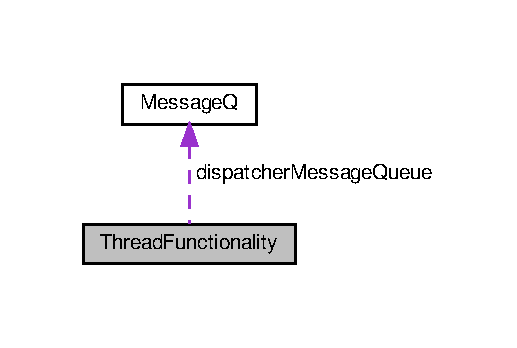
\includegraphics[width=248pt]{classThreadFunctionality__coll__graph}
\end{center}
\end{figure}
\subsection*{Static Public Member Functions}
\begin{DoxyCompactItemize}
\item 
\mbox{\Hypertarget{classThreadFunctionality_aa74339ed85a8193e09faf43b7fd648c8}\label{classThreadFunctionality_aa74339ed85a8193e09faf43b7fd648c8}} 
static void \hyperlink{classThreadFunctionality_aa74339ed85a8193e09faf43b7fd648c8}{dispatcher} (\hyperlink{classMessage}{Message} $\ast$message\+Ptr, unsigned long ID)
\begin{DoxyCompactList}\small\item\em Dispatcher-\/funktion, der håndterer indkommende events Disptacher-\/funktionen håndterer de beskeder, der er modtaget i programmets Message\+Queue. Dette gøres ved at switche på det modtagne event, som er defineret af den fælles protokol. \end{DoxyCompactList}\item 
\mbox{\Hypertarget{classThreadFunctionality_ac3e321db9529381c58a16abe25b8577e}\label{classThreadFunctionality_ac3e321db9529381c58a16abe25b8577e}} 
static void $\ast$ \hyperlink{classThreadFunctionality_ac3e321db9529381c58a16abe25b8577e}{dispatcher\+Thread\+Func} (void $\ast$arg)
\begin{DoxyCompactList}\small\item\em Kører dispatcher-\/funktionen i et \textquotesingle{}receive-\/handle-\/delete\textquotesingle{}-\/loop. \end{DoxyCompactList}\end{DoxyCompactItemize}


The documentation for this class was generated from the following files\+:\begin{DoxyCompactItemize}
\item 
thread\+Functionality.\+hpp\item 
thread\+Functionality.\+cpp\end{DoxyCompactItemize}

\hypertarget{structuserDeleteRide}{}\section{user\+Delete\+Ride Struct Reference}
\label{structuserDeleteRide}\index{user\+Delete\+Ride@{user\+Delete\+Ride}}


Inheritance diagram for user\+Delete\+Ride\+:\nopagebreak
\begin{figure}[H]
\begin{center}
\leavevmode
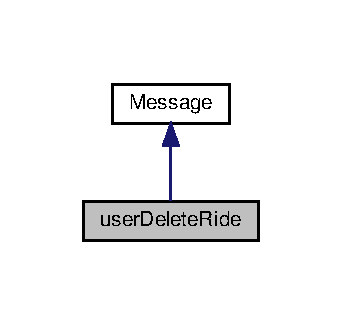
\includegraphics[width=164pt]{structuserDeleteRide__inherit__graph}
\end{center}
\end{figure}


Collaboration diagram for user\+Delete\+Ride\+:\nopagebreak
\begin{figure}[H]
\begin{center}
\leavevmode
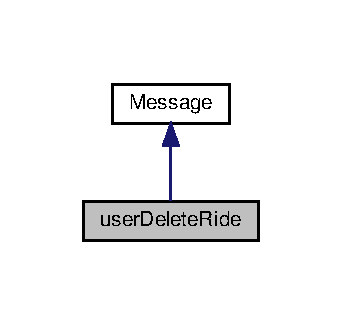
\includegraphics[width=164pt]{structuserDeleteRide__coll__graph}
\end{center}
\end{figure}


The documentation for this struct was generated from the following file\+:\begin{DoxyCompactItemize}
\item 
thread\+Functionality.\+hpp\end{DoxyCompactItemize}

\hypertarget{classUserInterface}{}\section{User\+Interface Class Reference}
\label{classUserInterface}\index{User\+Interface@{User\+Interface}}
\subsection*{Public Member Functions}
\begin{DoxyCompactItemize}
\item 
\mbox{\Hypertarget{classUserInterface_ae6fb70370701b3bd6120e923df9705b0}\label{classUserInterface_ae6fb70370701b3bd6120e923df9705b0}} 
\hyperlink{classUserInterface_ae6fb70370701b3bd6120e923df9705b0}{User\+Interface} ()
\begin{DoxyCompactList}\small\item\em Klassens constructor. Har ingen funktionalitet, men er deklareret for en sikkerheds skyld. \end{DoxyCompactList}\item 
\mbox{\Hypertarget{classUserInterface_ae588b2ff1711a016dd4c6fc5002c0841}\label{classUserInterface_ae588b2ff1711a016dd4c6fc5002c0841}} 
\hyperlink{classUserInterface_ae588b2ff1711a016dd4c6fc5002c0841}{$\sim$\+User\+Interface} ()
\begin{DoxyCompactList}\small\item\em Klassens destructor Har ingen funktionalitet, men er deklareret for en sikkerheds skyld. \end{DoxyCompactList}\item 
void \hyperlink{classUserInterface_a5a42468e90a1bbd89f6465ee11d56e93}{U\+I\+Receive\+To\+Dispatcher} (string event)
\begin{DoxyCompactList}\small\item\em Modtager events fra brugerfladen Kaldes af User\+Interface\+::\+U\+I\+Receive og evaluerer eventets type på baggrund af den overordnede protokol for E\+D\+Bike. Eventet og relevant data sendes derefter videre til dispatcher-\/tråden via Message\+Queue. \end{DoxyCompactList}\item 
bool \hyperlink{classUserInterface_a899642cb1d73de5804ac8b56d92ca94c}{validate\+Pin} (string input\+Pin)
\begin{DoxyCompactList}\small\item\em Validerer P\+IN, der er indtastet af bruger i client browser. \end{DoxyCompactList}\item 
\mbox{\Hypertarget{classUserInterface_a80c3e5e03d4f7d57d339badb4cf1eae6}\label{classUserInterface_a80c3e5e03d4f7d57d339badb4cf1eae6}} 
void \hyperlink{classUserInterface_a80c3e5e03d4f7d57d339badb4cf1eae6}{U\+I\+Receive} ()
\begin{DoxyCompactList}\small\item\em Lytter efter data fra brugerflade i client browser. Indeholder en overloaded version af Hub\+::on\+Message lampda-\/funktionen fra u\+Web\+Sockets-\/biblioteket. Denne funktion kører som en tråd og lytter efter events fra client browser og kalder User\+Interface\+::\+U\+I\+Receive\+To\+Dispatcher, når der modtages et event. \end{DoxyCompactList}\item 
void \hyperlink{classUserInterface_a44b574eb614bb90bb370f027ce88b8ea}{send\+To\+UI} (string event)
\begin{DoxyCompactList}\small\item\em Sender event til brugerflade i client browser Sender en string til brugerflade i client browser via u\+Web\+Sockets-\/funktionen Hub\+\_\+\+::broadcast. \end{DoxyCompactList}\item 
\mbox{\Hypertarget{classUserInterface_add59ee8e8c6cd74bd89dc1b529e5db95}\label{classUserInterface_add59ee8e8c6cd74bd89dc1b529e5db95}} 
void $\ast$ \hyperlink{classUserInterface_add59ee8e8c6cd74bd89dc1b529e5db95}{pin\+Timer} ()
\begin{DoxyCompactList}\small\item\em Blokerer for tjek af P\+I\+N-\/kode i 5 minutter Køres som en tråd og blokerer for validering af P\+IN i 5 minutter, når den kaldes. Når de 5 minutter er gået sættes antallet af resterende P\+I\+N-\/forsøg til 5. \end{DoxyCompactList}\item 
bool \hyperlink{classUserInterface_a569c725b82d4ba420574f072e0bfc866}{validate\+Wheel\+Size} (string wheel\+\_\+input)
\begin{DoxyCompactList}\small\item\em Validerer den indtastede hjulstørrelse Tjekker om den indtastede hjulstørrelse overholder en række regler. \end{DoxyCompactList}\end{DoxyCompactItemize}
\subsection*{Static Public Member Functions}
\begin{DoxyCompactItemize}
\item 
static void $\ast$ \hyperlink{classUserInterface_a29bcf3e43b86bda0fcfb9b3bfce93308}{call\+Pin\+Timer} (void $\ast$arg)
\begin{DoxyCompactList}\small\item\em Kalder User\+Interface\+::pin\+Timer Denne funktion gør det muligt at kalde pin\+Timer() (Tabel 10) som en tråd fra andre medlemsklasser, og fungerer altså som ’limen’ mellem de andre medlemsfunktioner og den egentlige pin\+Timer-\/metode. Grunden er, atstd\+::thread i C++ skal kaldes på statiske medlemsfunktioner. Denne funktion returnerer en pointer til pin\+Timer-\/metoden for objekt, der gives med som argument. \end{DoxyCompactList}\end{DoxyCompactItemize}


\subsection{Member Function Documentation}
\mbox{\Hypertarget{classUserInterface_a29bcf3e43b86bda0fcfb9b3bfce93308}\label{classUserInterface_a29bcf3e43b86bda0fcfb9b3bfce93308}} 
\index{User\+Interface@{User\+Interface}!call\+Pin\+Timer@{call\+Pin\+Timer}}
\index{call\+Pin\+Timer@{call\+Pin\+Timer}!User\+Interface@{User\+Interface}}
\subsubsection{\texorpdfstring{call\+Pin\+Timer()}{callPinTimer()}}
{\footnotesize\ttfamily static void$\ast$ User\+Interface\+::call\+Pin\+Timer (\begin{DoxyParamCaption}\item[{void $\ast$}]{arg }\end{DoxyParamCaption})\hspace{0.3cm}{\ttfamily [static]}}



Kalder User\+Interface\+::pin\+Timer Denne funktion gør det muligt at kalde pin\+Timer() (Tabel 10) som en tråd fra andre medlemsklasser, og fungerer altså som ’limen’ mellem de andre medlemsfunktioner og den egentlige pin\+Timer-\/metode. Grunden er, atstd\+::thread i C++ skal kaldes på statiske medlemsfunktioner. Denne funktion returnerer en pointer til pin\+Timer-\/metoden for objekt, der gives med som argument. 


\begin{DoxyParams}{Parameters}
{\em arg} & Void-\/pointer, som castes til User\+Interface\+::\+Pintimer \\
\hline
\end{DoxyParams}
\begin{DoxyReturn}{Returns}
Returnerer static void for at kunne blive kaldt af std\+::thread-\/biblioteket 
\end{DoxyReturn}
\mbox{\Hypertarget{classUserInterface_a44b574eb614bb90bb370f027ce88b8ea}\label{classUserInterface_a44b574eb614bb90bb370f027ce88b8ea}} 
\index{User\+Interface@{User\+Interface}!send\+To\+UI@{send\+To\+UI}}
\index{send\+To\+UI@{send\+To\+UI}!User\+Interface@{User\+Interface}}
\subsubsection{\texorpdfstring{send\+To\+U\+I()}{sendToUI()}}
{\footnotesize\ttfamily void User\+Interface\+::send\+To\+UI (\begin{DoxyParamCaption}\item[{string}]{event }\end{DoxyParamCaption})}



Sender event til brugerflade i client browser Sender en string til brugerflade i client browser via u\+Web\+Sockets-\/funktionen Hub\+\_\+\+::broadcast. 


\begin{DoxyParams}{Parameters}
{\em event} & String der indeholder det event der skal sendes til brugerflade i client browser \\
\hline
\end{DoxyParams}
\mbox{\Hypertarget{classUserInterface_a5a42468e90a1bbd89f6465ee11d56e93}\label{classUserInterface_a5a42468e90a1bbd89f6465ee11d56e93}} 
\index{User\+Interface@{User\+Interface}!U\+I\+Receive\+To\+Dispatcher@{U\+I\+Receive\+To\+Dispatcher}}
\index{U\+I\+Receive\+To\+Dispatcher@{U\+I\+Receive\+To\+Dispatcher}!User\+Interface@{User\+Interface}}
\subsubsection{\texorpdfstring{U\+I\+Receive\+To\+Dispatcher()}{UIReceiveToDispatcher()}}
{\footnotesize\ttfamily void User\+Interface\+::\+U\+I\+Receive\+To\+Dispatcher (\begin{DoxyParamCaption}\item[{string}]{event }\end{DoxyParamCaption})}



Modtager events fra brugerfladen Kaldes af User\+Interface\+::\+U\+I\+Receive og evaluerer eventets type på baggrund af den overordnede protokol for E\+D\+Bike. Eventet og relevant data sendes derefter videre til dispatcher-\/tråden via Message\+Queue. 


\begin{DoxyParams}{Parameters}
{\em event} & String der indeholder det event der skal sendes til brugerfladen \\
\hline
\end{DoxyParams}
\mbox{\Hypertarget{classUserInterface_a899642cb1d73de5804ac8b56d92ca94c}\label{classUserInterface_a899642cb1d73de5804ac8b56d92ca94c}} 
\index{User\+Interface@{User\+Interface}!validate\+Pin@{validate\+Pin}}
\index{validate\+Pin@{validate\+Pin}!User\+Interface@{User\+Interface}}
\subsubsection{\texorpdfstring{validate\+Pin()}{validatePin()}}
{\footnotesize\ttfamily bool User\+Interface\+::validate\+Pin (\begin{DoxyParamCaption}\item[{string}]{input\+Pin }\end{DoxyParamCaption})}



Validerer P\+IN, der er indtastet af bruger i client browser. 

Tjekker, om den indtastede P\+IN stemmer overens med den korrekte P\+IN og kalder et P\+I\+N-\/timeout, (medlemsfunktionen pin\+Timer (Tabel 10)) hvis P\+IN er skrevet forkert 5 gange i brugerfladen. Antallet af brugte forsøg dekrementeres hver gang, funktionen kaldes med en forkert pin. 
\begin{DoxyParams}{Parameters}
{\em event} & String der indeholder den indtastede P\+IN som skal tjekkes. \\
\hline
\end{DoxyParams}
\begin{DoxyReturn}{Returns}
True, hvis den indtastede P\+IN stemmer overens med den korrekte P\+IN. False, hvis den indtastede P\+IN ikke stemmer overens med den korrekte P\+IN eller hvis P\+I\+N-\/timeoutet er aktivt. 
\end{DoxyReturn}
\mbox{\Hypertarget{classUserInterface_a569c725b82d4ba420574f072e0bfc866}\label{classUserInterface_a569c725b82d4ba420574f072e0bfc866}} 
\index{User\+Interface@{User\+Interface}!validate\+Wheel\+Size@{validate\+Wheel\+Size}}
\index{validate\+Wheel\+Size@{validate\+Wheel\+Size}!User\+Interface@{User\+Interface}}
\subsubsection{\texorpdfstring{validate\+Wheel\+Size()}{validateWheelSize()}}
{\footnotesize\ttfamily bool User\+Interface\+::validate\+Wheel\+Size (\begin{DoxyParamCaption}\item[{string}]{wheel\+\_\+input }\end{DoxyParamCaption})}



Validerer den indtastede hjulstørrelse Tjekker om den indtastede hjulstørrelse overholder en række regler. 

\begin{DoxyReturn}{Returns}
Returnerer en bool, der indikerer om hjulstørrelsen er godkendt 
\end{DoxyReturn}


The documentation for this class was generated from the following files\+:\begin{DoxyCompactItemize}
\item 
.\+atom-\/beautify.\+User\+Interface.\+hpp\item 
\hyperlink{UserInterface_8hpp}{User\+Interface.\+hpp}\item 
\hyperlink{UserInterface_8cpp}{User\+Interface.\+cpp}\end{DoxyCompactItemize}

\hypertarget{structuserUnlockTry}{}\section{user\+Unlock\+Try Struct Reference}
\label{structuserUnlockTry}\index{user\+Unlock\+Try@{user\+Unlock\+Try}}


Inheritance diagram for user\+Unlock\+Try\+:\nopagebreak
\begin{figure}[H]
\begin{center}
\leavevmode
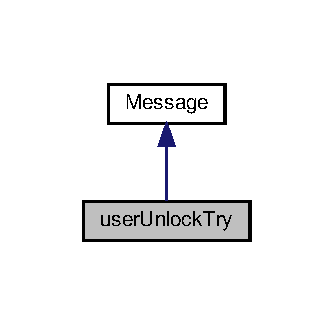
\includegraphics[width=160pt]{structuserUnlockTry__inherit__graph}
\end{center}
\end{figure}


Collaboration diagram for user\+Unlock\+Try\+:\nopagebreak
\begin{figure}[H]
\begin{center}
\leavevmode
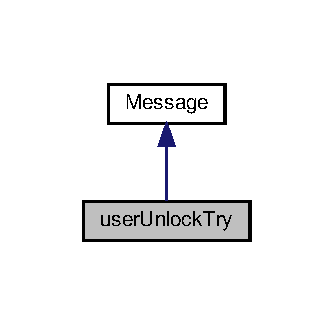
\includegraphics[width=160pt]{structuserUnlockTry__coll__graph}
\end{center}
\end{figure}


The documentation for this struct was generated from the following file\+:\begin{DoxyCompactItemize}
\item 
thread\+Functionality.\+hpp\end{DoxyCompactItemize}

\hypertarget{structwheelCircumference}{}\section{wheel\+Circumference Struct Reference}
\label{structwheelCircumference}\index{wheel\+Circumference@{wheel\+Circumference}}


Inheritance diagram for wheel\+Circumference\+:\nopagebreak
\begin{figure}[H]
\begin{center}
\leavevmode
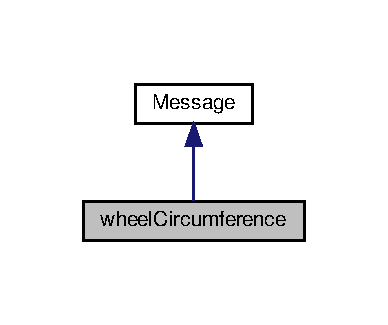
\includegraphics[width=186pt]{structwheelCircumference__inherit__graph}
\end{center}
\end{figure}


Collaboration diagram for wheel\+Circumference\+:\nopagebreak
\begin{figure}[H]
\begin{center}
\leavevmode
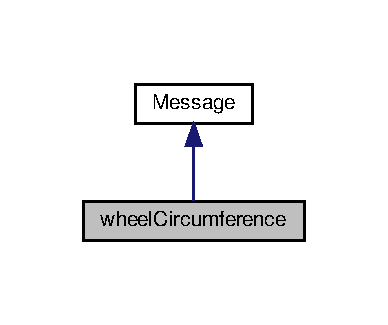
\includegraphics[width=186pt]{structwheelCircumference__coll__graph}
\end{center}
\end{figure}


The documentation for this struct was generated from the following file\+:\begin{DoxyCompactItemize}
\item 
thread\+Functionality.\+hpp\end{DoxyCompactItemize}

\chapter{File Documentation}
\hypertarget{DataBase_8cpp}{}\section{Data\+Base.\+cpp File Reference}
\label{DataBase_8cpp}\index{Data\+Base.\+cpp@{Data\+Base.\+cpp}}


Implementering af Data\+Basen.  


{\ttfamily \#include \char`\"{}Data\+Base.\+hpp\char`\"{}}\newline
Include dependency graph for Data\+Base.\+cpp\+:
\nopagebreak
\begin{figure}[H]
\begin{center}
\leavevmode
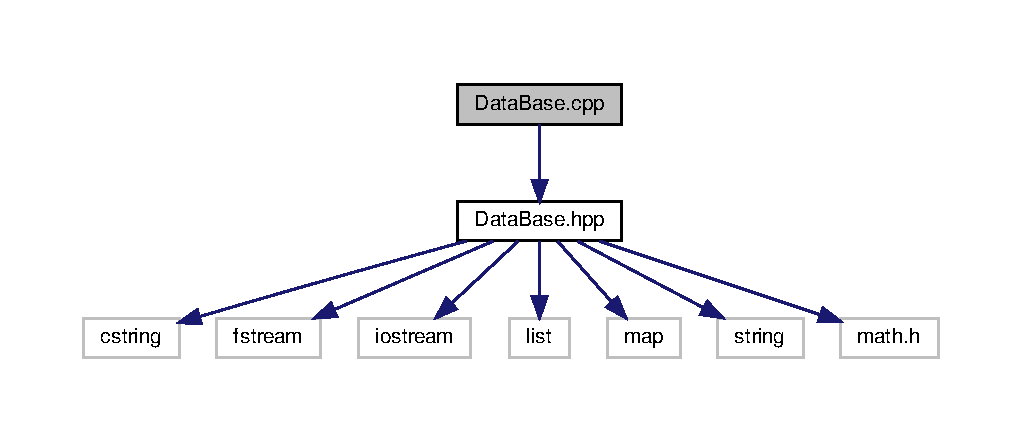
\includegraphics[width=350pt]{DataBase_8cpp__incl}
\end{center}
\end{figure}


\subsection{Detailed Description}
Implementering af Data\+Basen. 

Indeholder implementeringerne af funktionerne i Data\+Basen.

\begin{DoxyAuthor}{Author}
Frederik Runge-\/\+Dalager 

Ermin Obradovac 
\end{DoxyAuthor}
\begin{DoxyRefDesc}{Bug}
\item[\hyperlink{bug__bug000001}{Bug}]Hvis vi sletter en tur der ikke findes forsvinder hele Data\+Basen. \end{DoxyRefDesc}

\hypertarget{DataBase_8hpp}{}\section{Data\+Base.\+hpp File Reference}
\label{DataBase_8hpp}\index{Data\+Base.\+hpp@{Data\+Base.\+hpp}}


Funktionsprototyper til Data\+Basen.  


{\ttfamily \#include $<$cstring$>$}\newline
{\ttfamily \#include $<$fstream$>$}\newline
{\ttfamily \#include $<$iostream$>$}\newline
{\ttfamily \#include $<$list$>$}\newline
{\ttfamily \#include $<$map$>$}\newline
{\ttfamily \#include $<$string$>$}\newline
{\ttfamily \#include $<$math.\+h$>$}\newline
Include dependency graph for Data\+Base.\+hpp\+:
\nopagebreak
\begin{figure}[H]
\begin{center}
\leavevmode
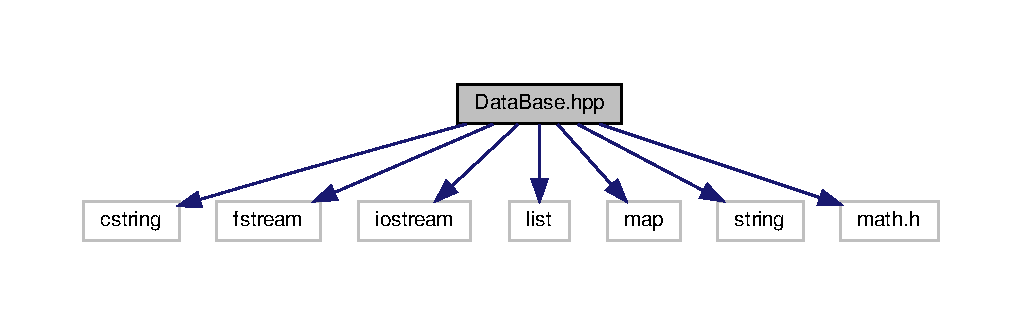
\includegraphics[width=350pt]{DataBase_8hpp__incl}
\end{center}
\end{figure}
This graph shows which files directly or indirectly include this file\+:
\nopagebreak
\begin{figure}[H]
\begin{center}
\leavevmode
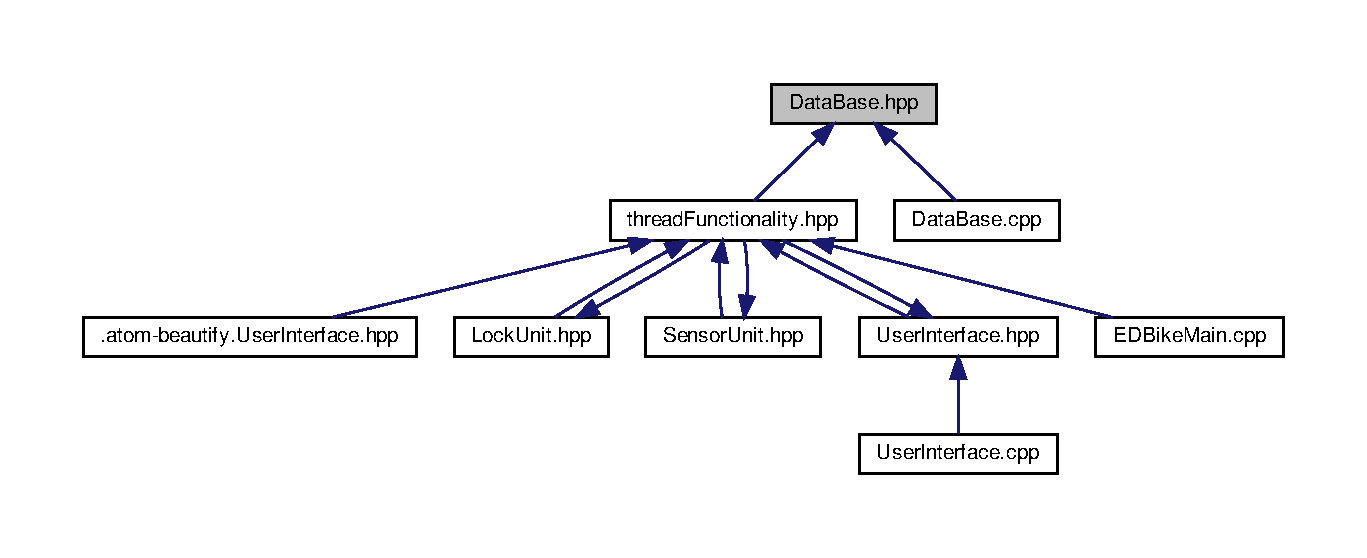
\includegraphics[width=350pt]{DataBase_8hpp__dep__incl}
\end{center}
\end{figure}
\subsection*{Classes}
\begin{DoxyCompactItemize}
\item 
class \hyperlink{classDataBase}{Data\+Base}
\end{DoxyCompactItemize}


\subsection{Detailed Description}
Funktionsprototyper til Data\+Basen. 

Indeholder prototyperne til funktionerne i Data\+Basen.

\begin{DoxyAuthor}{Author}
Frederik Runge-\/\+Dalager 

Ermin Obradovac 
\end{DoxyAuthor}
\begin{DoxyRefDesc}{Bug}
\item[\hyperlink{bug__bug000002}{Bug}]Hvis vi sletter en tur der ikke findes forsvinder hele Data\+Basen. \end{DoxyRefDesc}

\hypertarget{EDBikeMain_8cpp}{}\section{E\+D\+Bike\+Main.\+cpp File Reference}
\label{EDBikeMain_8cpp}\index{E\+D\+Bike\+Main.\+cpp@{E\+D\+Bike\+Main.\+cpp}}


Main-\/programmet for E\+D\+Bike.  


{\ttfamily \#include \char`\"{}thread\+Functionality.\+hpp\char`\"{}}\newline
{\ttfamily \#include $<$string$>$}\newline
Include dependency graph for E\+D\+Bike\+Main.\+cpp\+:
\nopagebreak
\begin{figure}[H]
\begin{center}
\leavevmode
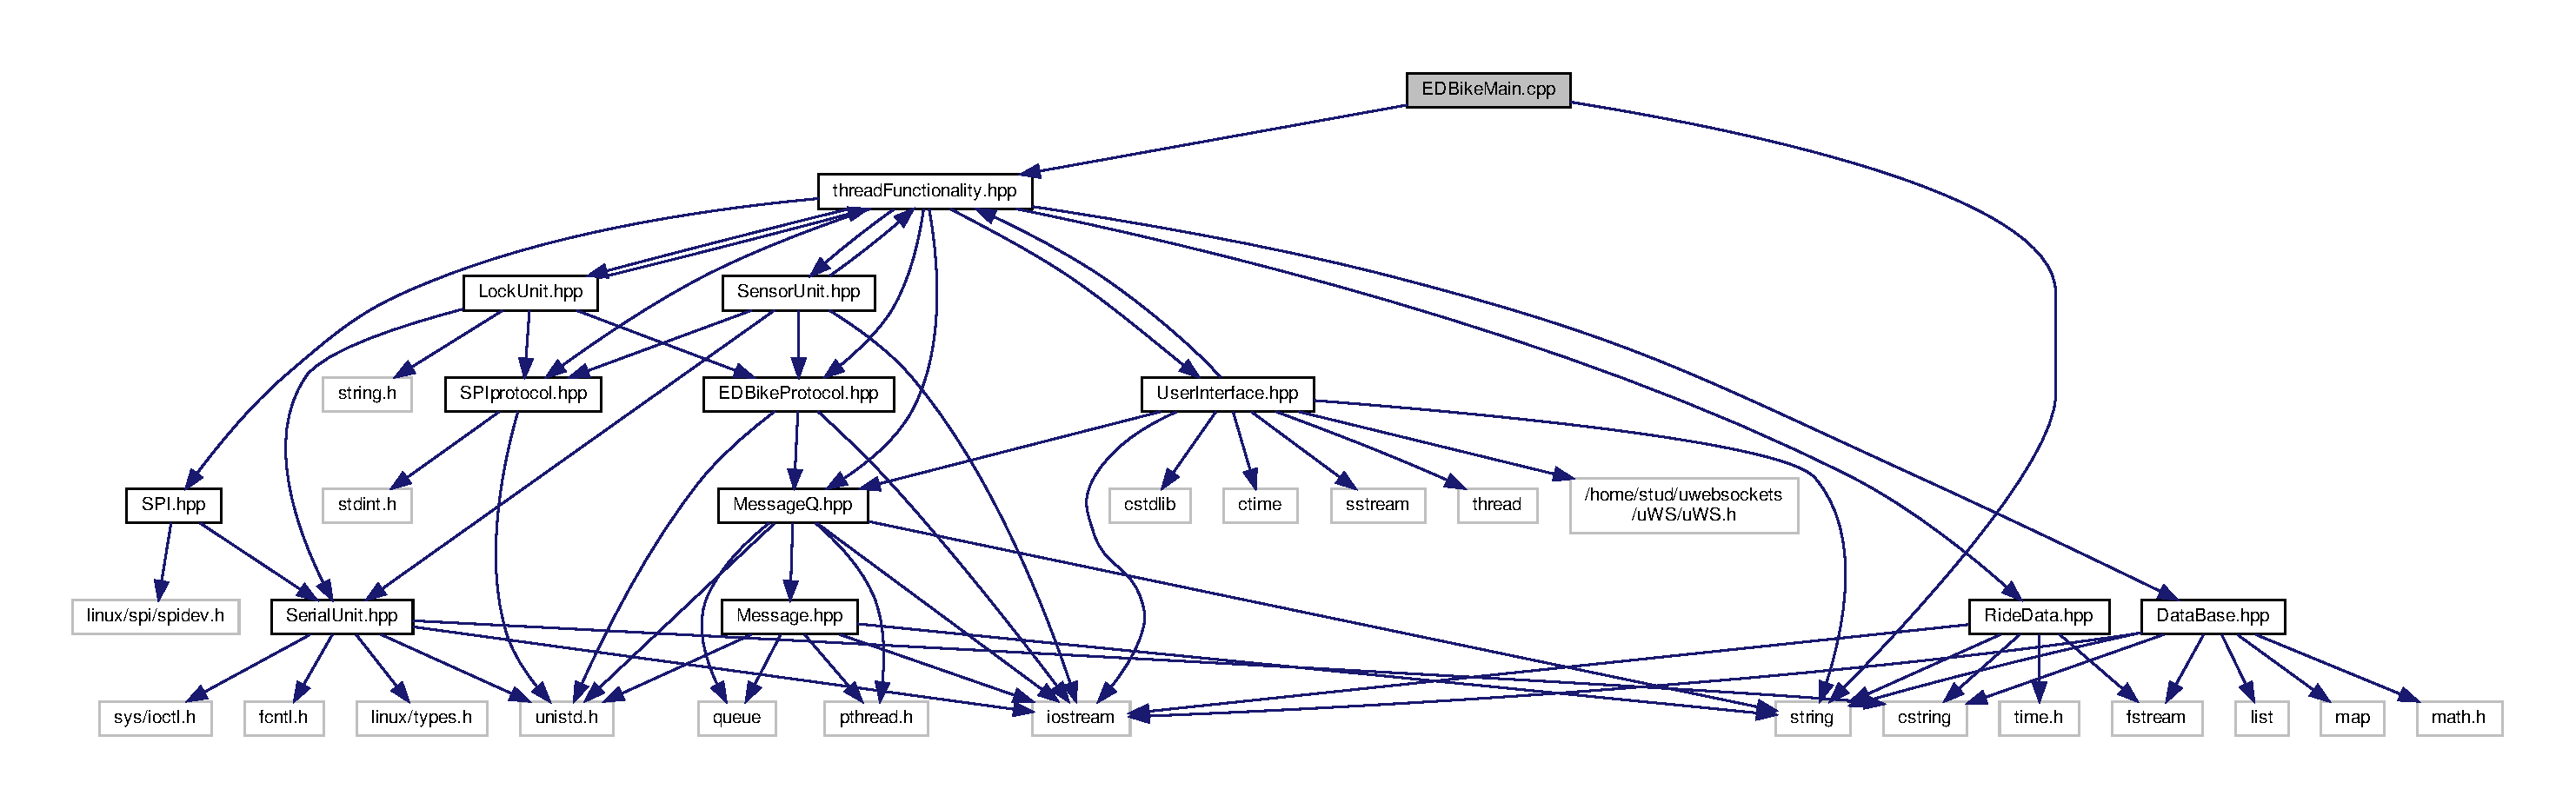
\includegraphics[width=350pt]{EDBikeMain_8cpp__incl}
\end{center}
\end{figure}


\subsection{Detailed Description}
Main-\/programmet for E\+D\+Bike. 

Starter de tre tråde U\+I\+Receiver, slave\+Puller og dispatcher\+Thread, som tilsammen håndterer E\+D\+Bike-\/funktionaliteten på R\+Pi.

\begin{DoxyAuthor}{Author}
Kristian Lau Jespersen 

Oskar Vedel 
\end{DoxyAuthor}
\begin{DoxyRefDesc}{Bug}
\item[\hyperlink{bug__bug000003}{Bug}]Ingen kendte bugs. \end{DoxyRefDesc}

\hypertarget{Message_8hpp}{}\section{Message.\+hpp File Reference}
\label{Message_8hpp}\index{Message.\+hpp@{Message.\+hpp}}


Implementation af Message-\/klassen Denne klasse implementerer en Message-\/klasse, der bruges som base-\/class til beskederne i systemet.  


{\ttfamily \#include $<$pthread.\+h$>$}\newline
{\ttfamily \#include $<$iostream$>$}\newline
{\ttfamily \#include $<$queue$>$}\newline
{\ttfamily \#include $<$string$>$}\newline
{\ttfamily \#include $<$unistd.\+h$>$}\newline
Include dependency graph for Message.\+hpp\+:\nopagebreak
\begin{figure}[H]
\begin{center}
\leavevmode
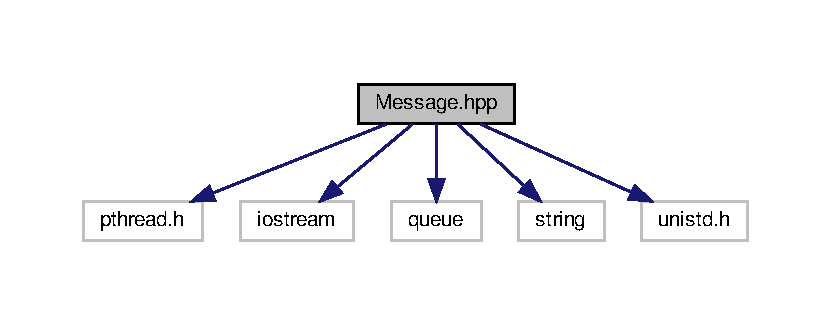
\includegraphics[width=350pt]{Message_8hpp__incl}
\end{center}
\end{figure}
This graph shows which files directly or indirectly include this file\+:
\nopagebreak
\begin{figure}[H]
\begin{center}
\leavevmode
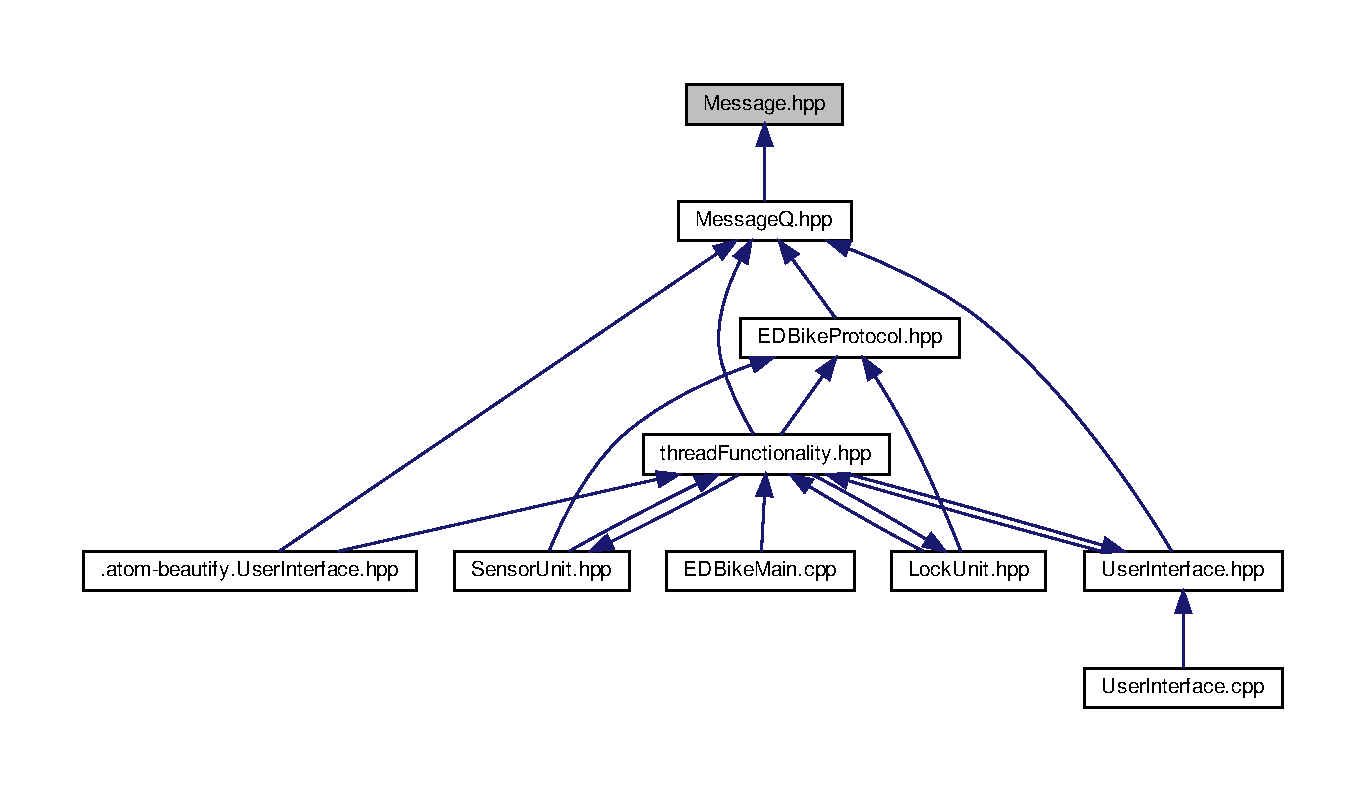
\includegraphics[width=350pt]{Message_8hpp__dep__incl}
\end{center}
\end{figure}
\subsection*{Classes}
\begin{DoxyCompactItemize}
\item 
class \hyperlink{classMessage}{Message}
\item 
struct \hyperlink{structitem}{item}
\end{DoxyCompactItemize}


\subsection{Detailed Description}
Implementation af Message-\/klassen Denne klasse implementerer en Message-\/klasse, der bruges som base-\/class til beskederne i systemet. 

\begin{DoxyAuthor}{Author}
Kristian Lau Jespersen 

Oskar Vedel 
\end{DoxyAuthor}
\begin{DoxyRefDesc}{Bug}
\item[\hyperlink{bug__bug000006}{Bug}]Ingen kendte bugs. \end{DoxyRefDesc}

\hypertarget{MessageQ_8hpp}{}\section{Message\+Q.\+hpp File Reference}
\label{MessageQ_8hpp}\index{Message\+Q.\+hpp@{Message\+Q.\+hpp}}


Implementation af Message\+Q-\/klassen Denne klasse implementerer en Message\+Queue, der bruges til at kommunikere mellem trådene i programmet.  


{\ttfamily \#include \char`\"{}Message.\+hpp\char`\"{}}\newline
{\ttfamily \#include $<$iostream$>$}\newline
{\ttfamily \#include $<$pthread.\+h$>$}\newline
{\ttfamily \#include $<$queue$>$}\newline
{\ttfamily \#include $<$string$>$}\newline
{\ttfamily \#include $<$unistd.\+h$>$}\newline
Include dependency graph for Message\+Q.\+hpp\+:\nopagebreak
\begin{figure}[H]
\begin{center}
\leavevmode
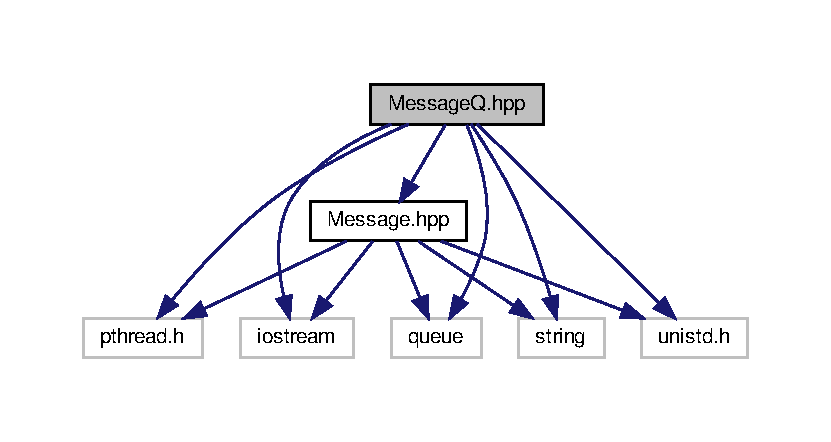
\includegraphics[width=350pt]{MessageQ_8hpp__incl}
\end{center}
\end{figure}
This graph shows which files directly or indirectly include this file\+:
\nopagebreak
\begin{figure}[H]
\begin{center}
\leavevmode
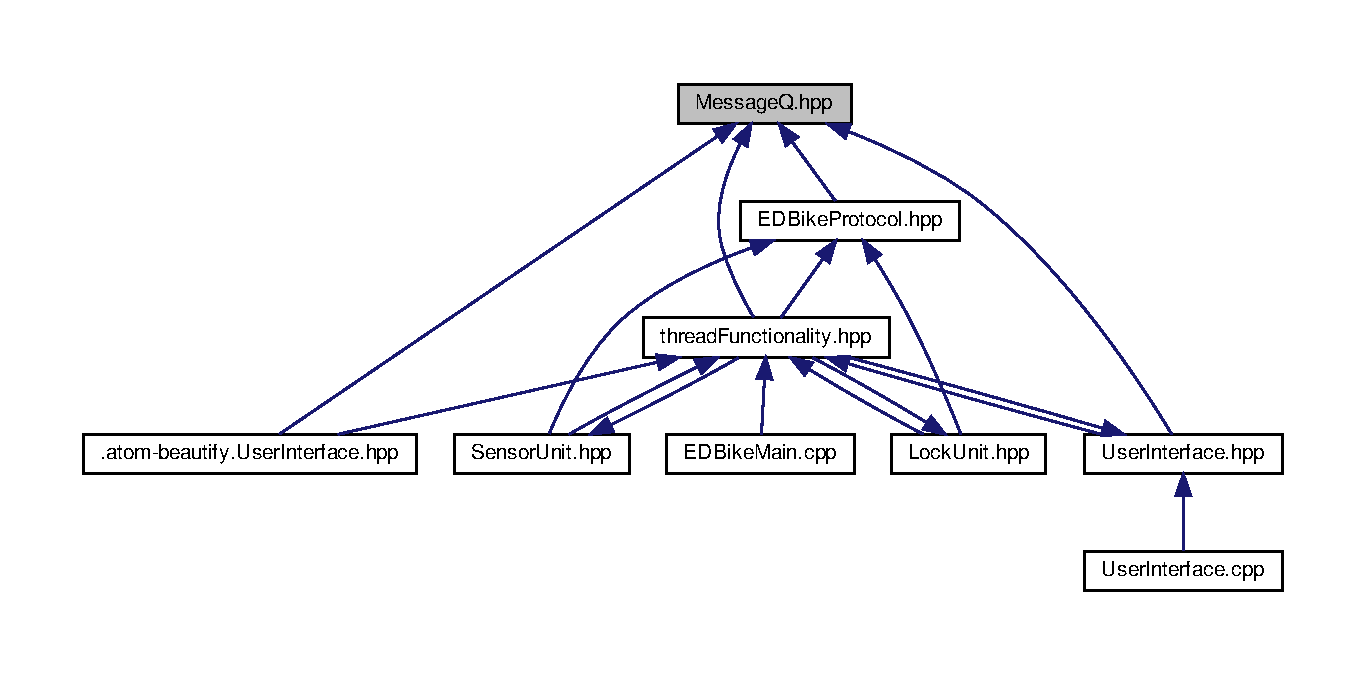
\includegraphics[width=350pt]{MessageQ_8hpp__dep__incl}
\end{center}
\end{figure}
\subsection*{Classes}
\begin{DoxyCompactItemize}
\item 
class \hyperlink{classMessageQ}{MessageQ}
\end{DoxyCompactItemize}


\subsection{Detailed Description}
Implementation af Message\+Q-\/klassen Denne klasse implementerer en Message\+Queue, der bruges til at kommunikere mellem trådene i programmet. 

\begin{DoxyAuthor}{Author}
Kristian Lau Jespersen 

Oskar Vedel 
\end{DoxyAuthor}
\begin{DoxyRefDesc}{Bug}
\item[\hyperlink{bug__bug000007}{Bug}]Ingen kendte bugs. \end{DoxyRefDesc}

\hypertarget{RideData_8cpp}{}\section{Ride\+Data.\+cpp File Reference}
\label{RideData_8cpp}\index{Ride\+Data.\+cpp@{Ride\+Data.\+cpp}}


Implementering af \hyperlink{classRideData}{Ride\+Data}.  


{\ttfamily \#include \char`\"{}Ride\+Data.\+hpp\char`\"{}}\newline
Include dependency graph for Ride\+Data.\+cpp\+:\nopagebreak
\begin{figure}[H]
\begin{center}
\leavevmode
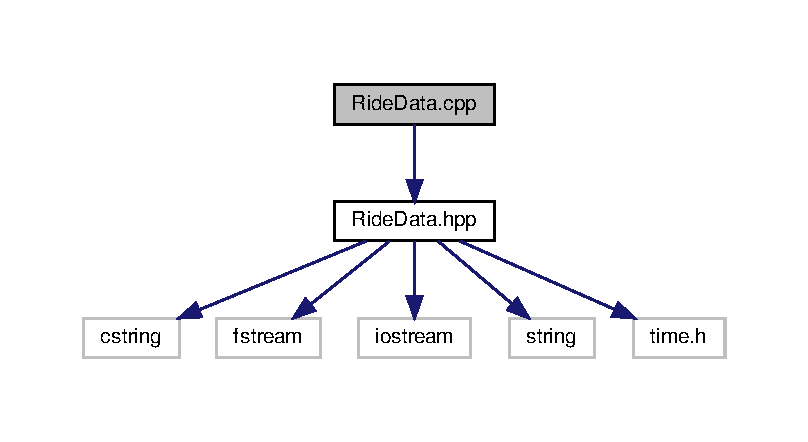
\includegraphics[width=350pt]{RideData_8cpp__incl}
\end{center}
\end{figure}


\subsection{Detailed Description}
Implementering af \hyperlink{classRideData}{Ride\+Data}. 

Indeholder implementeringerne af funktionerne i Ride\+Data-\/klassen.

\begin{DoxyAuthor}{Author}
Frederik Runge-\/\+Dalager 

Ermin Obradovac 
\end{DoxyAuthor}
\begin{DoxyRefDesc}{Bug}
\item[\hyperlink{bug__bug000008}{Bug}]Ingen kendte bugs. \end{DoxyRefDesc}

\hypertarget{RideData_8hpp}{}\section{Ride\+Data.\+hpp File Reference}
\label{RideData_8hpp}\index{Ride\+Data.\+hpp@{Ride\+Data.\+hpp}}


Funktionsprototyper til \hyperlink{classRideData}{Ride\+Data}.  


{\ttfamily \#include $<$cstring$>$}\newline
{\ttfamily \#include $<$fstream$>$}\newline
{\ttfamily \#include $<$iostream$>$}\newline
{\ttfamily \#include $<$string$>$}\newline
{\ttfamily \#include $<$time.\+h$>$}\newline
Include dependency graph for Ride\+Data.\+hpp\+:\nopagebreak
\begin{figure}[H]
\begin{center}
\leavevmode
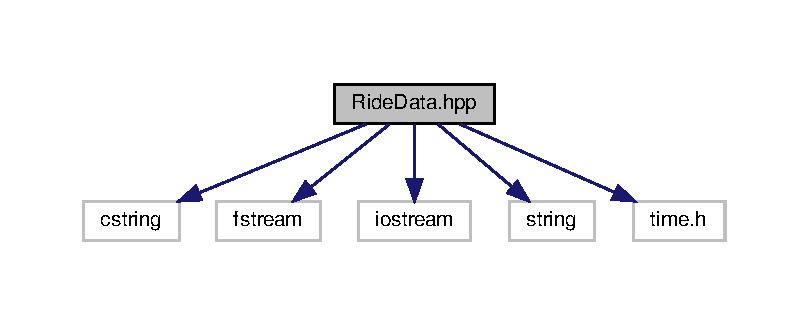
\includegraphics[width=350pt]{RideData_8hpp__incl}
\end{center}
\end{figure}
This graph shows which files directly or indirectly include this file\+:
\nopagebreak
\begin{figure}[H]
\begin{center}
\leavevmode
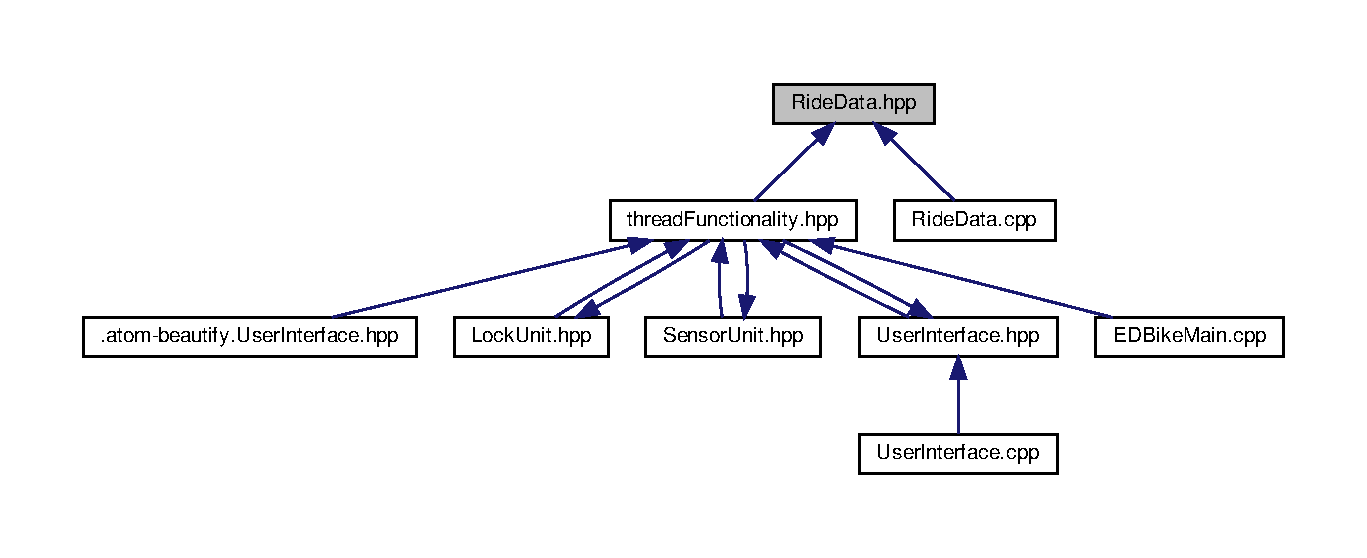
\includegraphics[width=350pt]{RideData_8hpp__dep__incl}
\end{center}
\end{figure}
\subsection*{Classes}
\begin{DoxyCompactItemize}
\item 
class \hyperlink{classRideData}{Ride\+Data}
\end{DoxyCompactItemize}


\subsection{Detailed Description}
Funktionsprototyper til \hyperlink{classRideData}{Ride\+Data}. 

Indeholder prototyperne til funktionerne i Ride\+Data-\/klassen

\begin{DoxyAuthor}{Author}
Frederik Runge-\/\+Dalager 

Ermin Obradovac 
\end{DoxyAuthor}
\begin{DoxyRefDesc}{Bug}
\item[\hyperlink{bug__bug000009}{Bug}]Ingen kendte bugs. \end{DoxyRefDesc}

\hypertarget{UserInterface_8cpp}{}\section{User\+Interface.\+cpp File Reference}
\label{UserInterface_8cpp}\index{User\+Interface.\+cpp@{User\+Interface.\+cpp}}


Implementation af \hyperlink{classUserInterface}{User\+Interface}.  


{\ttfamily \#include \char`\"{}User\+Interface.\+hpp\char`\"{}}\newline
Include dependency graph for User\+Interface.\+cpp\+:
\nopagebreak
\begin{figure}[H]
\begin{center}
\leavevmode
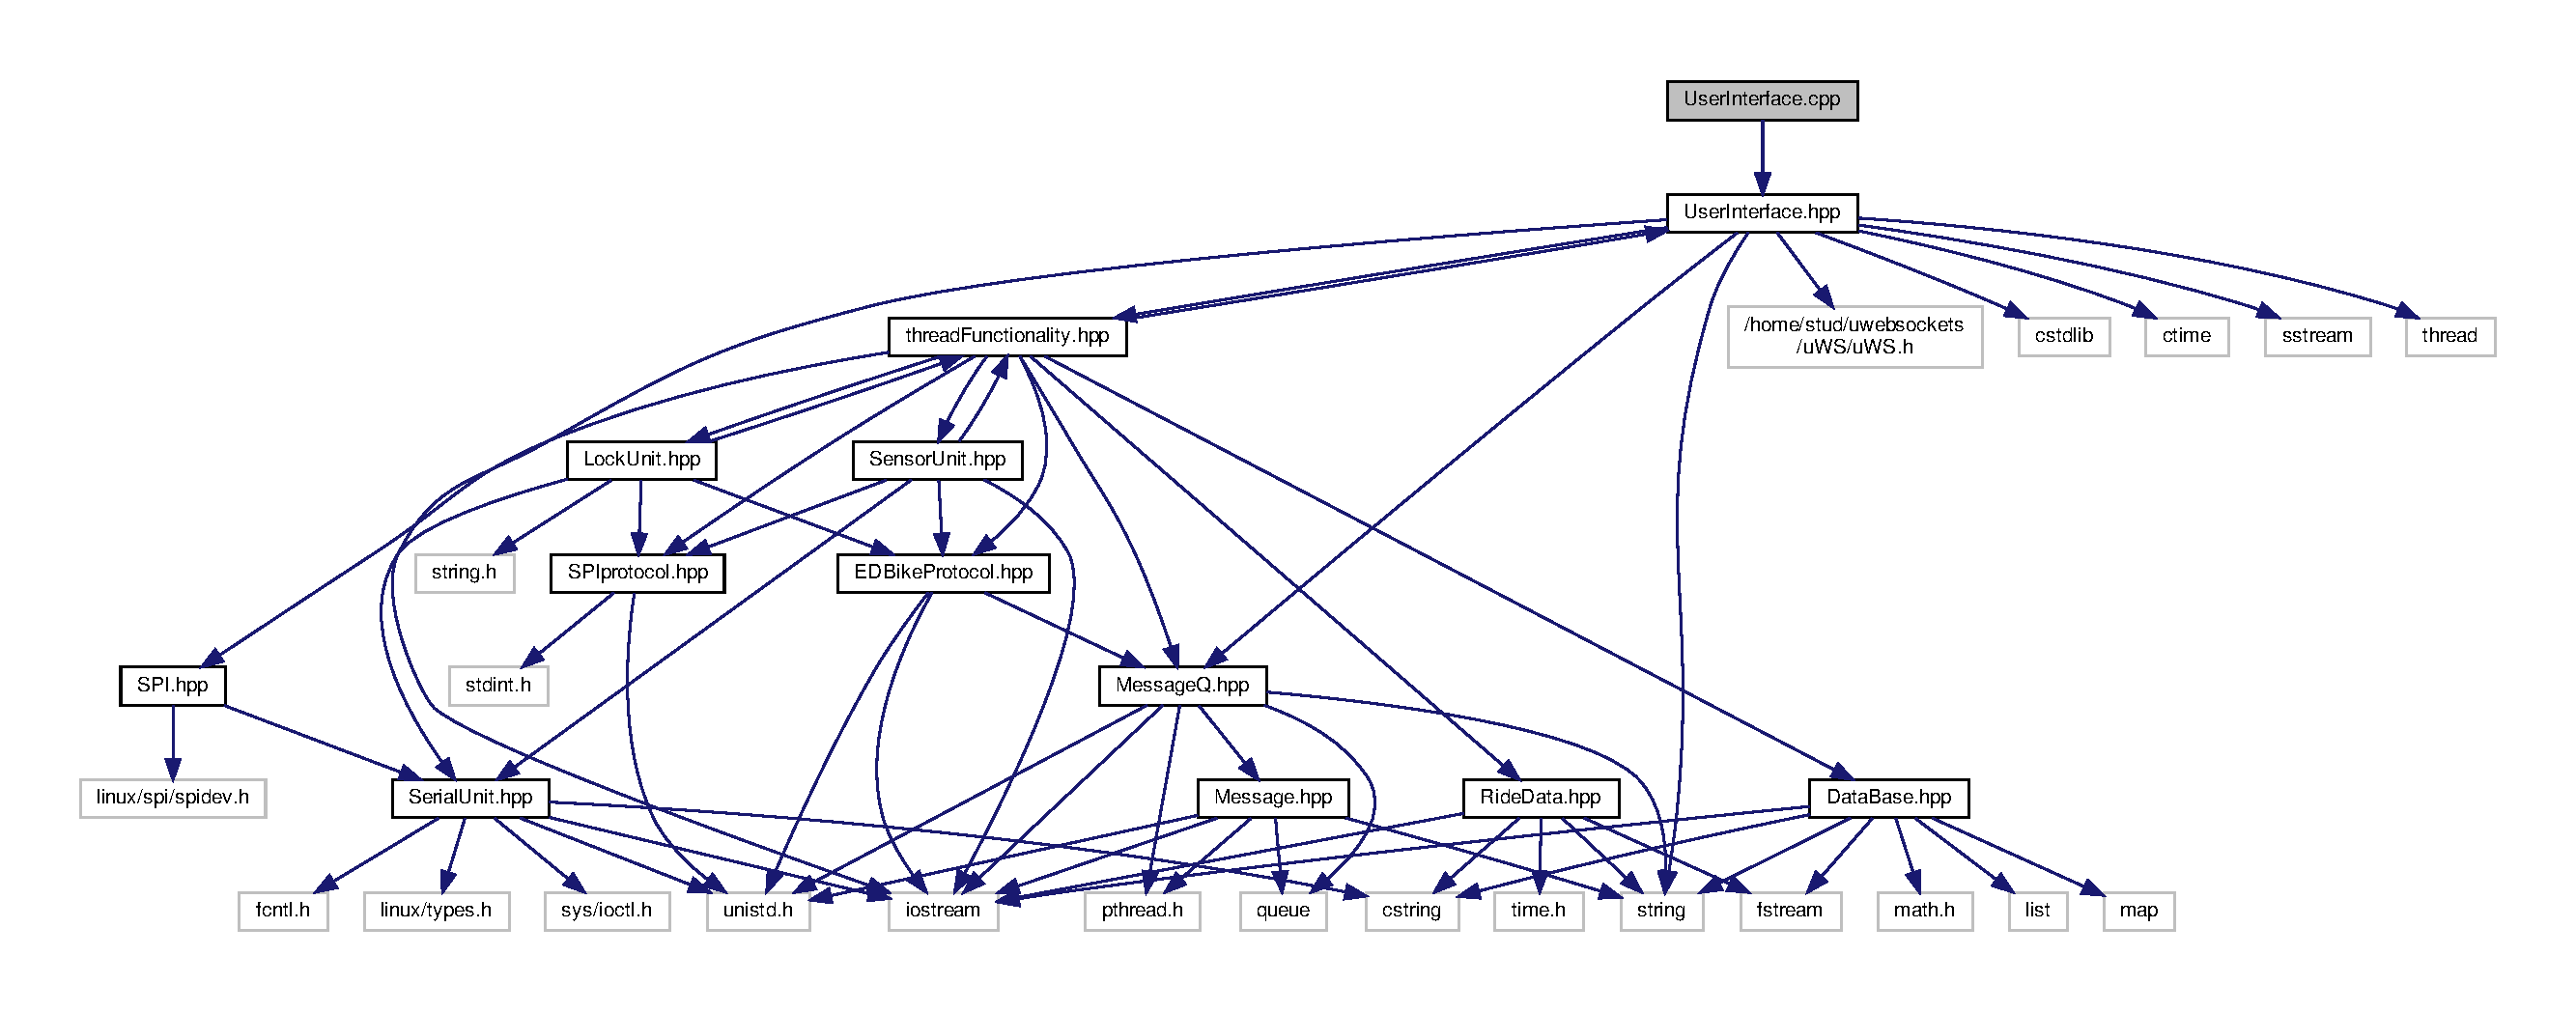
\includegraphics[width=350pt]{UserInterface_8cpp__incl}
\end{center}
\end{figure}


\subsection{Detailed Description}
Implementation af \hyperlink{classUserInterface}{User\+Interface}. 

Indeholder implementationer af medlemsfunktionerne i \hyperlink{classUserInterface}{User\+Interface}.

\begin{DoxyAuthor}{Author}
Sebastian Brahe 

Oskar Vedel 
\end{DoxyAuthor}
\begin{DoxyRefDesc}{Bug}
\item[\hyperlink{bug__bug000020}{Bug}]Det er muligt at indstille hjulstørrelsen til 0 \end{DoxyRefDesc}

\hypertarget{UserInterface_8hpp}{}\section{User\+Interface.\+hpp File Reference}
\label{UserInterface_8hpp}\index{User\+Interface.\+hpp@{User\+Interface.\+hpp}}


Funktionsprototyper til User\+Interface-\/klassen.  


{\ttfamily \#include \char`\"{}Message\+Q.\+hpp\char`\"{}}\newline
{\ttfamily \#include \char`\"{}thread\+Functionality.\+hpp\char`\"{}}\newline
{\ttfamily \#include $<$/home/stud/uwebsockets/u\+W\+S/u\+W\+S.\+h$>$}\newline
{\ttfamily \#include $<$cstdlib$>$}\newline
{\ttfamily \#include $<$ctime$>$}\newline
{\ttfamily \#include $<$iostream$>$}\newline
{\ttfamily \#include $<$sstream$>$}\newline
{\ttfamily \#include $<$string$>$}\newline
{\ttfamily \#include $<$thread$>$}\newline
Include dependency graph for User\+Interface.\+hpp\+:
\nopagebreak
\begin{figure}[H]
\begin{center}
\leavevmode
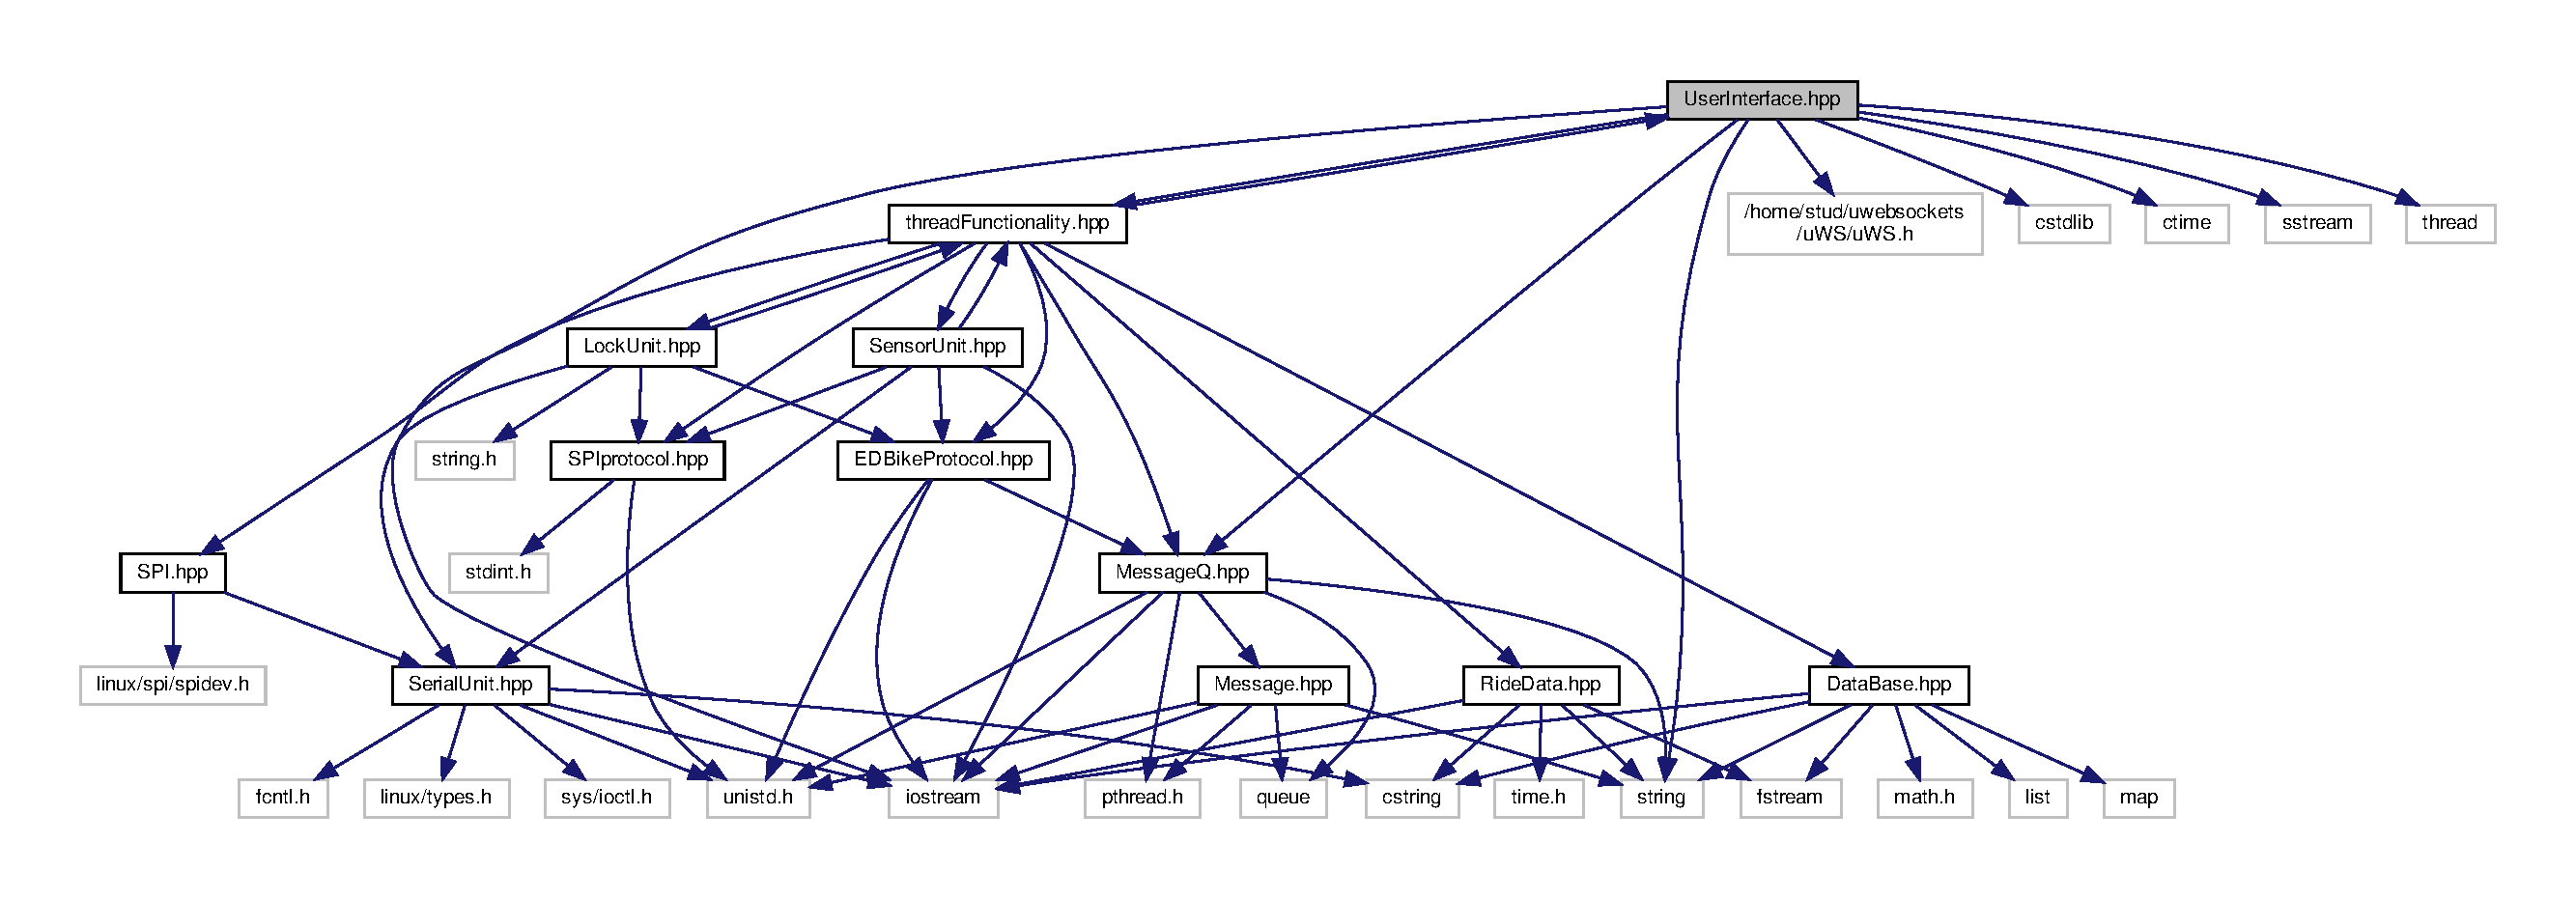
\includegraphics[width=350pt]{UserInterface_8hpp__incl}
\end{center}
\end{figure}
This graph shows which files directly or indirectly include this file\+:
\nopagebreak
\begin{figure}[H]
\begin{center}
\leavevmode
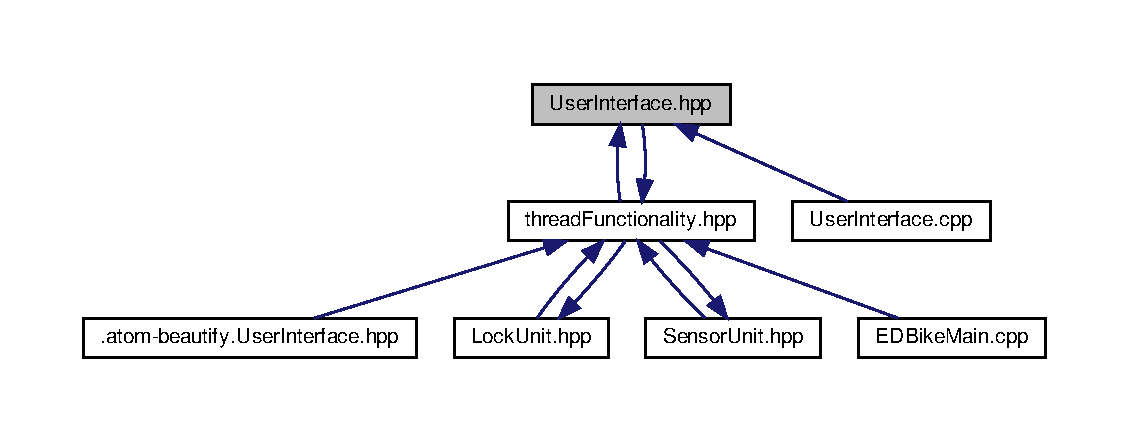
\includegraphics[width=350pt]{UserInterface_8hpp__dep__incl}
\end{center}
\end{figure}
\subsection*{Classes}
\begin{DoxyCompactItemize}
\item 
class \hyperlink{classUserInterface}{User\+Interface}
\end{DoxyCompactItemize}


\subsection{Detailed Description}
Funktionsprototyper til User\+Interface-\/klassen. 

Indeholder prototyperne til \hyperlink{UserInterface_8cpp}{User\+Interface.\+cpp}, der håndterer kommunikation mellem server og brugerflade.

\begin{DoxyAuthor}{Author}
Sebastian 

Oskar Vedel 
\end{DoxyAuthor}
\begin{DoxyRefDesc}{Bug}
\item[\hyperlink{bug__bug000021}{Bug}]Det er muligt at indstille hjulstørrelsen til 0 \end{DoxyRefDesc}

%--- End generated contents ---

% Index
\backmatter
\newpage
\phantomsection
\clearemptydoublepage
\addcontentsline{toc}{chapter}{Index}
\printindex

\end{document}
